\section{Einleitung}
%for reference to this section
\label{section:Introduction}
Ein wichtiger Teil von Webseiten, ist die Gestaltung und das Design. Um eine Seite nach dem Design zu gestalten, verwendet man im World Wide Web das CSS 3. \newline
Seit ein paar Jahren, werden sogenannte Präprozessoren für CSS entwickelt, die Erweiterungen zu CSS bereitstellen.\newline
Was sind nun Präprozessoren? Wie werden sie verwendet und welche Erweiterungen stellen Sie im Detail zur Verfügung?
Diese Fragen sollen in der Arbeit behandelt werden.\newline
Mit CSS3 ist schon eine große Vielfalt an Gestaltungen möglich. CSS3 bietet einfache Berechnungen und es gibt Funktionen, mit denen Beispielsweise die Ecken einer Box abgerundet werden können oder einem Hintergrund ein Verlauf gegeben wird.
Die Notwendigkeit, der Verwendung von Präprozessoren für CSS, wird immer größer, da die Ansprüche an die Gestaltung von Webseiten immer mehr Bedeutung bekommt. Folgende Abbildung zeigt das Suchinteresse nach den Suchbegriffen Less, Sass, Styuls und Css in Google:\footnote[1]{Google Trends zum Vergleich von Suchinteresse zu Less, Sass, Stylus und CSS:  http://www.google.at/trends/explore\#geo=US\&q=sass,+less,+stylus,+css\&cmpt=q.}\newline
\begin{figure}[h]
	\centering
	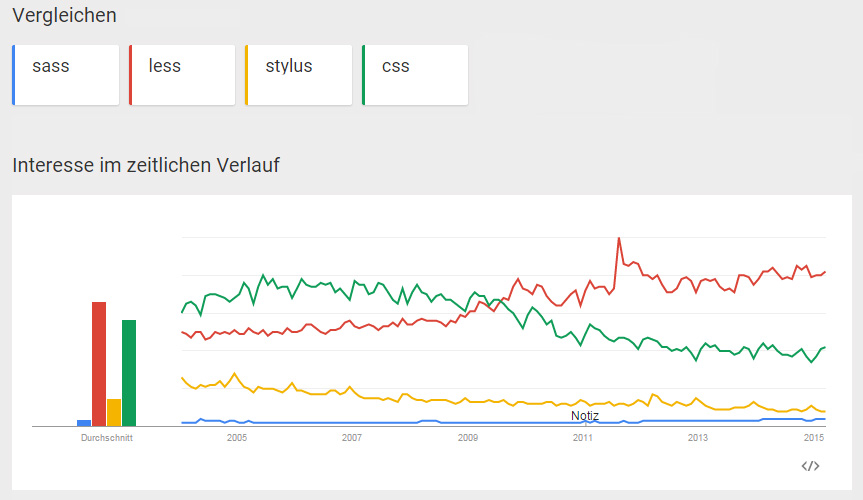
\includegraphics[height=8.0cm]{images/GoogleTrends_less_vs_sass_vs_stylus_vs_css.jpg}
	\caption{
		Suchtrends in Google nach Sass, Less, Styuls und Css
	}
	%for reference to this figure
	\label{figure:Trends Google}
\end{figure}
Die Statistik in der Abbildung zeigt das Interesse im zeitlichen Verlauf von 2005 bis 2015. \newline
In der Abbildung ist gut zu erkennen, dass das Interesse nach Less gerade in den letzten 5 Jahren sehr gestiegen ist. Trotzallem wird noch sehr oft nach CSS gesucht, was darauf zurückfzuführen ist, dass, trotz den Vorteilen von CSS-Präprozessoren, noch sehr viele Programmierer/innen mit einfachem CSS3 ihre Seiten stylen. \newline
Wie die Abbildung zeigt, werden im Vergleich zu Less und Css selten Suchanfragen zu Sass und Stylus über Google abgesetzt.\newline
Die Statistik die sich über die Abbildung ergibt, spiegelt jedoch nur das Suchinteresse über Google wieder und kann nicht als wissenschaftlich erwiesene Statistik zur Verwendung der gezeigten Programmiersprachen gesehen werden.\newline
Die Abbildung zeigt, dass Less noch vor CSS nachgefragt wird. Less ist einer der bekanntesten CSS-Präprozessoren, der wie Sass und Stylus in dieser Arbeit behandelt wird. \newline
CSS-Präprozessoren bieten viele Erweiterungen, welche die Erstellung eines Webseitenstylings vereinfachen und den Workflow bei der Erstellung verringern. Neben den Erweiterungen der Präprozessoren, gibt es für die CSS-Präprozessoren viele Tasks in Node.js, die dabei helfen, die Verwendung der Präprozessoren mit Hilfe von Grunt oder Gulp noch weiter zu Verbessern. \newline
Der Praktische Teil dieser Arbeit wird mittels solcher Grunttaks realisiert, wie das im Detail umgesetzt wird, wird in Kapitel 6 beschrieben.\newline
\subsection{Forschungsfrage}
%for references to this subsection
\label{subsection:Coding}
In dieser Arbeit soll die Frage:
\begin{quote}
\glqq{} Welche Präprozessoren gibt es und wie funktionieren diese? Wie funktionieren Präprozessoren im Generellen? \grqq{}
\end{quote}
beantwortet werden.\newline
Die Relevanz dieser Frage wird im zunehmenden Interesse, Webseiten immer besser und stylischer zu gestalten, gesehen. Die Webseiten sollen immer innovativer und kreativer werden und oft reicht es nicht mehr, mit den von CSS3 gebotenen Möglichkeiten auszukommen.\newline
In dieser Arbeit soll nun, wie schon unter Punkt 1 erläutert, untersucht werden, welche Tools bereitgestellt werden, um CSS3 zu erweitern und den Ansprüchen zu entsprechen.\newline
Am Beginn der Arbeit wird kurz erläutert wie sich Präprozessoren definieren und welchen Anteil am Gesamten die einzelnen Bestandteile, wie z.B. Mixins und Vererbung, haben und wie diese zusammenwirken. Im nächsten Schritt wird auf die einzelnen Methoden eingegangen um im Anschluss, im praktischen Teil der Arbeit, eine Library mit den beschriebenen CSS-Präprozessoren zu erstellen. 

\subsection{Aufbau}
Wie in Punkt 2 beschrieben wird in der Arbeit zuerst auf die Grundthematik Präprozessoren eingegangen und beschrieben, wie Präprozessoren im Gesamten funktionieren und die Bestandteile im Einzelnen verwendet und erstellt werden.\newline
Als Nächstes wird erklärt welche Auswirkungen Präprozessoren auf die Erstellung eines Webseitenstylings haben. Das Kapitel dient zur Information der Leser/innen und um die technischen Weiterfürhungen der Präprozessoren in den weiteren Kapiteln besser verstehen zu können.\newline
Das Unterkapitel 2.1 erläutert kurz den Begriff Workflow, da dieser in der Arbeit des öfteren verwendet wird.\newline
Die weiteren Unterkapitel 2.3 bis 2.5 erläutern im Speziellen die genannten CSS-Präprozessoren Less, Sass und Stylus, nachdem in Kapitel 2.2 noch genauer auf Software Komponenten eingegangen wird.\newline 
In Kapitel 3 wird auch kurz auf den Begriff Superset eingegangen.\newline
Nachdem auch die Präprozessoren Less, Sass und Stylus erläutert werden, wird im Weiteren in Kapitel 4 darauf eingegangen, was Parsing ist und wie das im Speziellen bei den erwähnten Präprozessoren funktioniert.\newline
Nach dieser Einführung wird die Benützung und Implementierung der, in Punkt 1 genannten Tools beschrieben. \newline
Kapitel 5 beschreibt die genaue Verwendung der in Kapitel 2.6 beschriebenen Erweiterungen.
Nach der Theoretischen Einführung in das Thema, beschreibt Kapitel 6 die Umsetzung und Realisierung des praktischen Teils.\newline
Im letzten Kapitel wird noch einmal auf die Vorteile von CSS-Präprozessoren eingegangen und diese mit dem praktischen Teil der Arbeit verglichen und so herausgearbeitet, wie sich diese Vorteile auf die Arbeit mit CSS-Präprozessoren auswirken.
\newpage
\section{Was sind CSS-Präprozessoren}
Präprozessoren sind Computerprogramme, welche Daten vorbereiten und zur Weiterverarbeitung an ein anderes Programm weitergeben. In den meisten Fällen, wird ein Präprozessor dazu verwendet, Eingabedaten, im Falle dieser Arbeit CSS-Styles, zu konvertieren.\autocite[]{Peter.2012}\newline
Präprozessoren werden benützt um beispielsweise Variabilität zu schaffen. Im Falle dieser Arbeit wird Variabilität in Bezug auf die mehrfache Verwendung gleicher Codeabschnitte in einem Stylesheet verstanden. Bspw. die Schriftart oder Schriftfarbe.
In dieser Arbeit geht es um die CSS-Präprozessoren Sass, Less und Stylus. Diese Präprozessoren werden eingesetzt, um das Schreiben des Codes sowie die Syntax zu erleichtern. Desweiteren stellen sie Funktionen und Variablen zur Verfügung. \newline
Mithilfe der genannten Präprozessoren können Aufgaben automatisiert werden. Es gibt die Möglichkeit Variablen zu erstellen und so die Bearbeitung von Stylings wie z.B. der Farbe, um ein Vielfaches zu erleichtern. Möchte man in einem CSS file die Farbe der Schrift verändern, muss man alle Stellen suchen, an denen diese Farbe zugeordnet wird. Verwendet man beispielsweise mit less eine Variable für die Farbe, so muss nur an einer Stelle, dort wo die Farbe der Variablen zugewiesen wird, die Farbe geändert werden.\newline
Nicht nur Variablen sondern auch Funktionen und Mixins werden von CSS-Präprozessoren bereit gestellt. Im Gegensatz zu einfachem CSS kann man mit den genannten Präprozessoren Mixins erstellen, die dabei helfen den Code übersichtlicher zu Gestalten. Mit einem Mixin kann z.B. ein Clearfix erstellt werden. Hierfür wird folgender Code, in scss syntax, siehe Kapitel 2.3 für die Definition von SCSS, erstellt:
\begin{lstlisting}[
	float=h,
	caption=erstellen eines Mixins (scss),
]
@mixin .clearfix {
 content: ".";
  display: block;
  height: 0;
  clear: both;
  visibility: hidden;
}

.mainContent {
  @include: .clearfix;
}
\end{lstlisting}
\newline
Die Zeilen 1 bis 7 in Listening 1 erstellen das Mixin \textit{clearfix} und in Zeile 10 wird gezeigt, wie dieses dann aufgerufen werden kann. Mit diesem Mixin kann vermieden werden, dass die in dem Mixin enthaltenen Stylings jedes mal erneut erstellt werden müssen. Stattdessen kann an jeder gewünschten Stelle im Code mit dem Befehl ''include:clearfix" der gesamte Codeabschnitt eingebunden werden.

Ein weiterer Vorteil von CSS-Präprozessoren ist, dass der Code verschachtelt werden kann. Folgendes Listing zeigt, wie sich das verschachteln des Codes auf die Lesbarkeit auswirken kann. Listing 2 zeigt den Code ohne Verschachtelung und Listing 3 mit Verschachtelung:\newline
\begin{lstlisting}[
	float=h,
	caption= Code ohne Verschachtelung (css),
]
#content .text .title{
  font-size: 12px;
  color: #dedede;
  font-weight: normal;
}
#content .text .title h1{
  font-size: 18px;
  color: #ffffaa;
  font-weight: bold;
}
#content .text .title h3{
  color: #efefef;
}
\end{lstlisting}

\begin{lstlisting}[
	caption= Code mit Verschachtelung (scss),
]
#content .text{
  .title{
    font-size: 12px;
    color: #dedede;
    font-weight: normal;
    h1{
      font-size: 18px;
      color: #ffffaa;
      font-weight: bold;
    }
    h3{
      color: #efefef;
    }
  }
}
\end{lstlisting}

Wie in den 2 Listings erkennbar, ist der Sinn von CSS-Präprozessoren nicht immer, den Code zu verkürzen, sondern die Schreibweise und dadurch auch die Lesbarkeit des Codes zu vereinfachen. In Listing 2 wird Zeile 1 in den Zeilen 6 und 11 wiederholt. Dies ist in Listing 3 nicht der Fall. Durch die Verschachtelung können beliebig viele Klassen, die sich innerhalb der Klasse text befinden, angesprochen werden, ohne dass immer alle darüberliegenden Klassen aufgerufen werden müssen. \newline
Es sollte jedoch darauf geachtet werden, dass es nicht immer sinnvoll ist, den Code zu verschachteln. Hat man z.B. einen Button, der auf der ganzen Seite immer grün sein soll, macht es keinen Sinn, dem Button die Styles in einer Verschachtelung zu geben, da man dann immer darauf achten muss, dass der Button auch wirklich in diesem Abschnitt des Quellcodes auftritt. Stattdessen ist es hier sinnvoller, den Button separat zu stylen und bei etwaigen Änderungen, diese dann in der Verschachtelung anzuführen.

Neben den genannten Erweiterungen von Less, Sass und Stylus zu CSS kann man zusätzlich den Workflow verbessern, wie der Workflow verbessert werden kann, wird in Kapitel 2.1 beschrieben. Werden die Präprozessoren richtig verwendet kann der Code sauberer und auch kürzer gehalten werden.\newline
Durch den Einsatz der Erweiterungen, kann ein komplexer Code vereinfacht werden, wodurch der Code wartbarer und übersichtlicher wird. Auch kann der Zeitaufwand für die Erstellung der Stylesheets verkürzt werden, da Beispielsweise ein Code, der häufig verwendet wird, mithilfe eines Mixins nur einmal definiert werden muss.

Der Code von CSS-Präprozessoren ist immer valides CSS, da die Präprozessoren Erweiterungen von CSS darstellen. Die am Beginn des Kapitels genannten Präprozessoren sind drei der bekanntesten CSS-Präprozessoren, es gibt jedoch noch weitere, wie zum Beispiel Turbine oder Switch CSS \autocite[]{Jung.2010}.

Um zu überprüfen, ob das geschriebene Stylesheet valide und von guter Qualität ist, gibt es Linting, dies ist die Überprüfung von CSS auf Validität und Codequalität. Es gibt einige OpenSource Tools, die die Überprüfung des Stylesheets einfach und schnell ermöglichen. Ein gutes OpenSource Tool ist z.B. CSSLint von Nicolas C. Zakas und Nicole Sullivan\footnote[2]{open source Tool zur Überprüfung von CSS: https://github.com/CSSLint/csslint/wiki/About.}\newline
Neben der Überprüfung der Codequalität werden mit Linting auch die Browserperformance und viele weitere Punkte wie z.B.
\begin{itemize}
  \item Parsing Fehler
  \item leere Anweisungen
  \item Nullwerte benötigen keine Einheiten
  \item keine IDs in Selektoren
  \item nicht zu viele Floats verwenden
  \item nicht zu viele Schriften verwenden
\end{itemize} 
gecheckt. \newline\newline
Wie zuvor beschrieben, bieten CSS-Präprozessoren einige Vorteile, können jedoch auch Nachteile haben,  wenn sie falsch verwendet werden. Diese Arbeit vergleicht die 3 bekanntesten CSS-Präprozessoren, jedoch nicht mit dem Ziel herauszufinden, welche Variante die Beste ist, da es keinen \grqq{besten Präprozessor}\glqq{} gibt.\newline
Welchen Präprozessor man verwendet bzw. benötigt liegt im Interesse jedes einzelnen. Hier einige Meinungen, von Programmierern, die mit Less, Sass bzw. Scss oder Stylus arbeiten. 
\begin{quote}
``Less, because it is intuitive and also is the engine inside Twitter Bootstrap. So if you want to edit Bootstrap CSS you edit using Less."(Stephanie Hughes, zitiert nach \cite[]{psdtowp.2014})
\end{quote} 
\begin{quote}
``I use LESS as a CSS preprocessor. ... I like it because it's closest to vanilla CSS. This way, if you find yourself in a situation where you have to fix something in pure CSS, you haven't forgotten how to do so, by working in LESS.

In general, I'm a big fan of preprocessors. They allow you to programmatically style your site or app, and they make writing clean, DRY, Object-Oriented CSS much easier."(Jamie Marcus, zitiert nach \cite[]{psdtowp.2014})
\end{quote} 
\begin{quote}
``I have surrendered to SCSS …it has the best tooling support (including Chrome) and the most devs using it. I *really* like the others too and have zero qualms about them."(Brian Leroux, zitiert nach \cite[]{psdtowp.2014})
\end{quote} 
\begin{quote}
``I use Scss because most projects use it and Stylus on my own projects. I'm really fond of the stylus syntax, the fact that it makes my stack 100\% JavaScript and find that it's by far the fastest compiler."(Wes Bos, zitiert nach \cite[]{psdtowp.2014})
\end{quote} 
Aus den Zitaten geht klar hervor, dass auf Grund vieler Vorlieben und Beweggründe ein bestimmter CSS-Präprozessor gewählt wird. \newline
Die Wahl des CSS-Präprozessors hängt auch von der eigenen Arbeitsweise und den Anforderungen durch die Projekte an den CSS-Präprozessor selbst ab.\newline

Um das Schreiben eines Stylesheets noch weiter zu vereinfachen, gibt es nicht nur die genannten Präprozessoren, sondern auch Postprozessoren wie \glqq{}Autoprefixer\grqq{}. Ein Autoprefixer erlaubt es, im Stylesheet auf die prefixes für die verschiedenen Browser zu verzichten und diese dann mithilfe des Autoprefixers automatisch hinzuzufügen. Ein Autoprefixer verwendet eine Datenbank mit allen gängigen browsern und fügt alle prefixes für diese Browser automaitsch hinzu.
Nachfolgender Code zeigt ein Beispiel, wie ein Autoprefixer funktioniert.
\begin{lstlisting}[
	caption= Verwendung Autoprefixer (css),
]
//css code without prefixes
a {
  transition: transform 1s
}

//css code after autoprefixer
a {
  -webkit-transition: -webkit-transform 1s;
  transition: -ms-transform 1s;
  transition: transform 1s
}
\end{lstlisting}
Ein Autoprefixer kann mithilfe von Grunt, welches in dieser Arbeit im praktischen Teil verwendet wird, installiert und auf das geschriebene Stylesheet angewendet werden. Ein Autoprefixer kann sowohl auf css-code als auch auf scss, less oder stylus Code angewendet werden.\newline
Um den Autoprefixer in grunt zu verwenden, wird folgender Code in das Gruntfile.js geschrieben:\autocite[]{Sitnik.2013}
\begin{lstlisting}[
	caption= Code in Gruntfile für Autoprefixer,
]
autoprefixer: {
  dist: {
    files: {
      'build/style.css': 'style.css'
    }
  }
},
watch: {
  styles: {
    files: ['style.css'],
    tasks: ['autoprefixer']
  }
}
...
grunt.loadNpmTasks('grunt-autoprefixer');
\end{lstlisting}
Wie beschrieben, kann der Autoprefixer mit Grunt verwendet werden. Grunt ist ein Tool, mithilfe dessen, Tasks automatisch, also ohne zutun des Benutzers, der Benutzerin ablaufen. Grunt wird mit npm, dem node package manager, installiert.\newline
Die Installation erfolgt über die Kommandozeile. Bevor Grunt installiert werden kann, muss jedoch npm installiert sein.\newline
Um die Verwendung von grunt zu erleichtern, benötigt man die Kommandozeilenschnittstelle von Grunt. Wird diese Schnittstelle verwendet, kann grunt von jedem Ordner aus aufgerufen werden. Es ist aber auch möglich grunt von der Shell, die von Windows zur Verfügung gestellt wird, aufzurufen.\newline\newline
Um Grunt zu verwenden, benötigt man eine package.json und ein Gruntfile.js.\newline
Ein Beispiel für eine package.json und ein Gruntfile.js:
\begin{lstlisting}[
	caption= Beispiel package.json,
]
{
  "name": "my-project-name",
  "version": "0.1.0",
  "devDependencies": {
    "grunt": "~0.4.5",
    "grunt-contrib-jshint": "~0.10.0",
    "grunt-contrib-nodeunit": "~0.4.1",
    "grunt-contrib-uglify": "~0.5.0"
  }
}
\end{lstlisting}
Im Abschnitt der \glqq{}devDependencies\grqq{} wird angegeben, welche grunt-tasks installiert sein müssen. 
\begin{lstlisting}[
	caption= Beispiel Gruntfile.js,
]
module.exports = function(grunt) {

  // Project configuration.
  grunt.initConfig({
    pkg: grunt.file.readJSON('package.json'),
    uglify: {
      options: {
        banner: '/*! <%= pkg.name %> <%= grunt.template.today("yyyy-mm-dd") %> */\n'
      },
      build: {
        src: 'src/<%= pkg.name %>.js',
        dest: 'build/<%= pkg.name %>.min.js'
      }
    }
  });

  // Load the plugin that provides the "uglify" task.
  grunt.loadNpmTasks('grunt-contrib-uglify');

  // Default task(s).
  grunt.registerTask('default', ['uglify']);

};
\end{lstlisting}
Nachdem grunt installiert wurde und die package.json und das Gruntfile.js richtig befüllt wurden, müssen die packages, welche in der package.json unter \glqq{}devDependencies\grqq{} angegeben wurden, installiert werden. \newline
Hat man das CLI, also die Kommandozeilenschnittstelle, von Grunt installiert, werden alle benötigten packages automatisch beim aufruf von grunt installiert, da das CLI bei jedem Aufruf von grunt überprüft, ob nicht installierte packages benötigt werden.\newline
Verwendet man die normale windows shell, muss man vor dem grunt-Aufruf noch \glq{}npm install\grq{}  ausführen. Mit diesem Aufruf von npm werden alle benötigten Packages mit einem Durchlauf installiert.\newline
Im praktischen Teil der Arbeit wird grunt verwendet und das Kapitel 6 beschreibt die Verwendung von Grunt noch genauer.\newline
Das gelesene Kapitel beschreibt den Nutzen und die Verwendung von CSS-Präprozessoren. Es soll erläutern, welche Vorteile und Nachteile so ein Präprozessor bietet. Im nächsten Kapitel wird der Begriff Workflow genauer definiert.
\subsection{Workflow}
Was ist Workflow? Wie wird Workflow definiert?\newline
Diese Fragen werden in folgendem Kapitel erörtert und beantwortet.\newline
\begin{quote}
"Workflow ist ein Arbeitsablauf... Mit dem Workflow können Geschäftsprozesse, an denen Mitarbeiter aus mehreren Abteilungen in einer vorgegebenen Reihenfolge beschäftigt sind, informationstechnisch realisiert werden. Die einzelnen Aktivitäten eines Workflows stehen in einem logischen Zusammenhang und einer zeitlichen Abfolge zueinander. "
\autocite[]{ITWissen.info.2014}
\end{quote}
Das Zitat beschreibt, dass ein Workflow eine Abfolge von Aktivitäten ist. In Zusammenhang mit dieser Arbeit, bedeudet Workflow die Ausführung verschiedener Arbeitsschritte in einer definierten Abfolge.\newline
Der erste Arbeitsschritt bei der Erstellung eines Webseitenstylings ist die Erstellung eines Stylesheets. In dieser Arbeit werden less, sass und stylus behandelt. Es wird also entweder eine style.less, eine style.sass bzw. style.scss oder eine style.styl erstellt. \newline
Durch die Verwendung von Präprozessoren, kann schon bei der Erstellung des Stylesheets der Workflow vereinfacht und verbessert werden, da durch Erweiterungen wie bspw. Variablen und Mixins, das schreiben des Codes erleichtert wird.\newline
Neben der erwähnten Erweiterungen kann der Workflow zusätzlich noch durch die Verwendung von Molekülen verbessert werden.

Unter einem Molekül wird, wie auch in der Chemie, eine Zusammensetzung von Atomen verstanden. \newline
In Bezug auf CSS sind Atome einzelne Stylings wie bspw. ein Inputfeld oder ein Submitbutton. Durch die Zusammensetzung der Atome kann ein Molekül, bei diesem Beispiel ein Formular, erstellt werden.\autocite[]{Frost.2013}\newline
Mithilfe der Moleküle, können Abschnitte von Stylings einmal für die gesamte Seite erstellt werden, und müssen so nicht wiederholt definiert werden.

Um diese Styles richtig auf der Webseite ausgeben zu können, folgt der nächste Arbeitsschritt. Die Kompilierung der Dateien in CSS.\newline
Für die Kompilierung gibt es für jeden der genannten CSS-Präprozessoren einige ThirdPartyLibraries wie z.B. Koala für Sass und Less oder CodeKit, welche less, stylus und sass kompiliert. \newline
Wie im vorherigen Absatz erwähnt, kann durch die Verwendung der Erweiterungen der Workflow verbessert werden, da der erste Arbeitsschritt schneller und verbessert durchgeführt werden kann. \newline
Die 2 genannten Libraries Koala und CodeKit ermöglichen es, die erstellten Stylesheets in Echtzeit zu kompilieren, so kann der Workflow ein weiteres mal verbessert werden, da die Erstellung des Stylesheets und dessen Kompilierung parallel ablaufen.\newline

Bei der Verwendung von CSS-Präprozessoren, wird in den meisten Fällen, wie auch bei der Benützung von CSS, nur die erstellte css Datei im HTML-Code eingebunden. Um die Stylings zu verändern, muss bspw. bei Stylus, die Stylesheetdatei .styl bearbeitet und erneut kompiliert werden um die Änderungen zu sehen. \newline
Um direkt in den Developer Tools, das CSS bearbeiten und ändern zu können, wird von den Präprozessoren die Möglichkeit für CSS-SourceMaps bereitgestellt. Sogenannte SourceMap-Dateien, sind json-Dateien, welche ein Mapping zwischen den kompilierten CSS Deklarationen und dem Sourcefile, also der ursprünglichen Stylesheetdatei, definiert. Durch diese Datei wird es ermöglicht, dass im Developer Tool von Chrome direkt der CSS Code verändert werden kann. Um die SourceMap-Datei im Chrome verwenden zu können, muss die Verwendung in den Developer Tools aktiviert werden. Nach der Aktivierung, wird die generierte CSS-Datei bei jeder Änderung in den Developer Tools automatisch neu geladen.\newline
Durch die Verwendung von SourceMaps kann der Workflow noch einmal verbessert werden, da nicht für jede Änderung die Quelldatei bearbeitet werden muss.\autocite[]{developer.2013}

Nachdem in den vorangegangenen Absätzen die Vor- und Nachteile von Präprozessoren erläutert wurden, wird im nächsten Kapitel genauer auf den Begriff  \glqq{}Software Komponenten\grqq{} eingegangen.
\newpage
\subsection{Software Komponenten}
Software Komponenten (im weiteren Verlauf als Komponenten bezeichnet) sind wiederverwendbare Bausteine einer Applikation, welche aus Software-Code bestehen. Komponenten implementieren spezifische Funktionalitäten gemeinsam mit vordefinierten Schnittstellen. Da es sich um wiederverwendbare Teile eines Codes handelt, sind Komponenten sogenannte Software-Bausteine, die einen bestimmten Bereich eines Geschäftsfeldes kapseln, jedoch keine abgeschlossene Applikation darstellen, und nicht für sich alleine ablaufen können. \autocite[1]{Andresen.2003}\newline
In Bezug auf diese Arbeit, sind bspw. Mixins Komponenten von CSS-Präprozessoren. Diese Komponente kann wiederverwendet werden und bildet einen eigenschändigen Bereich des CSS-Präprozessors. Wie beschrieben, ist sie jedoch keine abgeschlossene Applikation und kann aus diesem Grund nicht alleine Ablaufen.

Im Buch von Andreas Andresen, Komponentenbasierte Softwareentwicklung, \autocite[2]{Andresen.2003} werden auf Seite 2 einige Vorteile von Komponenten aufgezählt. Die wichtigsten für diese Arbeit sind folgende:
\begin{enumerate}
  \item überschaubare Größenordnung
  \item trennen Zuständigkeiten
  \item einfach einsetzbar und kombinierbar
  \item einfach wiederverwendbar
  \item fördern eine schnelle Applikationsentwicklung
  \item einfach austauschbar
\end{enumerate} 
Dieselben Vorteile haben teilweise auch die Erweiterungen von CSS-Präprozessoren. Beispielsweise Mixins. Mixins können, wie schon erwähnt, im weitesten Sinne als Software Komponenten bezeichnet werden, da die Punkte aus der Aufzählung genau auf Mixins übertragen werden können. Mixins haben eine überschaubar Größenordnung, da sie meist nur eine Aufgabe erfüllen, wie z.B. einen Hintergrund mit Farbverlauf oder eine CSS-Transition zu erstellen.\newline
Ein Mixin erfüllt auch die Punkte 3, 4 und 6. Ein Mixin kann an jeder Stelle des Stylesheets verwendet werden und ist austauschbar, da einfach ein anderes Mixin verwendet werden kann. Ebenso kann es kombiniert werden, in dem 2 Mixins beim selben Selector aufgerufen werden.\newline
Somit hat ein Mixin alle bereits aufgezählten Vorteile einer Software Komponente. Jedocch gibt es auch Anforderungen an Komponenten \autocite[6]{Andresen.2003}. Folgende Aufzählung zeigt einige Anforderungen an die Architektur:
\begin{enumerate}
\item die Ermöglichung einer einfachen Kommunikation von Stytem und Komponente untereinander
\item komplexe Zusammenhänge innerhalb von Stystemen und zwischen Komponenten und Stystemen müssen auf übersichtliche und einfache Weise strukturiert werden können.
\item Komponenten und Stysteme müssen effizient dimensioniert werden
\item bestehende Komponentnen müssen einfach integrierbar sein
\item eine einfache Wiederverwendung der Komponenten muss ermöglicht werden
\item die Zuständigkeit muss klar getrennt sein.
\item das System muss die Anforderungen in Bezug auf Robustheit, Zuverlässigkeit, Performance, Sicherheit und Skalierbarkeit erfüllen.
\end{enumerate}
Bei den Anforderungen an die Architektur, kann ein Mixin nicht alle Punkte erfüllen. Die Punkte 4, 5, 6 können von Mixins erfüllt werden, da diese auch die größten Vorteile eines Mixins darstellen. Bei den anderen Punkten kann dies jedoch nicht ganz deutlich definiert werden. \newline
Ein Mixin als eine Erweiterung eines CSS-Präprozessors, muss diese Punkte nicht erfüllen, es gibt keine direkten Anforderungen an die Erweiterungen in diesem Sinne.\newline
Diese Kriterien legen nahe, dass ein Mixin nur im weiteren Sinne als eine Komponente bezeichnet werden können. Auch die anderen Erweiterungen von CSS-Präprozessoren können, wenn dann nur im weiteren Sinne als solche bezeichnet werden.\newline\newline
Nach dieser allgemeinen Einführung in CSS-Präprozessoren und der Erläuterung von Workflow und Software Komponenten, wird in den nächsten Kapiteln näher auf die, für diese Arbeit verwendeten, Präprozessoren im Speziellen eingegangen.
\newpage
\subsection{Superset} 
Ein Superset ist eine sogenannte Obermenge. Der Begriff Superset kommt aus der Mengenlehre und bedeutet, dass B ein Superset von A ist, sobald A in B enthalten ist. Bezogen auf diese Arbeit heißt das, dass Beispielsweise Scss, eine Syntax-Variante von Sass, ein Superset von CSS3 ist.\newline
Sobald das CSS3 valide ist, hat man auch ein valides, also gültiges SCSS. Umgekeht gilt das jedoch nicht.  Vorteilhaft ist, dass ein schon vorhandener CSS3-Code einfach weiterverwendet werden kann und mit SCSS erweiterbar ist. Um also eine vorhandene CSS3-Datei in SCSS umzuwandeln, muss nur die Dateiendung von .css auf .scss umgeschrieben werden.

Von den, in dieser Arbeit genannten, Programmiersprachen Less, Sass und Stylus ist nur die Syntax-Variante SCSS von Sass bzw. Less jeweils ein Superset von CSS. \newline
Der Begriff Superset darf nicht mit dem Begriff Erweiterung verwechselt werden.\newline
Bei einer Obermenge ist dessen Untermenge immer Valide für die Obermenge, das heißt bei einem Superset wie SCSS ist das CSS, die Untermenge, immer valides SCSS.\newline
Bei den Erweiterungen Sass und Stylus gilt dies jedoch nicht, da die Syntax dieser Präprozessoren nicht dieselbe von CSS3 ist. Auf die Syntax und die Unterschiede wird in den Kapiteln 4.1, 4.2 und 4.3 näher eingegangen.\newline\newline
Nach den Erläuterungen zu Less, Sass, Stylus und den Erweiterungen in den letzten Kapiteln, wird im nächsten Kapitel auf das Parsing im Allgemeinen und im Speziellen von Less, Sass und Stylus eingegangen.

\subsection{Parser}
Ein Parser ist ein Programm zur Zerlegung und Umwandlung einer beliebigen Eingabe, welche zur Weiterverarbeitung in ein brauchbares Fromat umgewandelt wird. Ein Parser erzeugt zusätzliche Strukturbeschreibungen und bedeutet Syntaxanalyse. \newline
Der Parser verwendet zur Analyse eines Textes einen lexikalischen Scanner, auch Lexer genannt. Ein Lexer zerlegt die Eingabe in sogenannte Tokens (beispielsweise Wörter oder Eingabesymbole) die der Parser versteht. \newline
Bei einem HTML Code würde der Lexer die Datei in HTML-Tags und Fließtext zerteilen und so an den Parser weiterleiten. Den Lexer interessiert nur das Aussehen der Syntaxelemente wie z.b. die spitzen Klammern eines Tags, während der Parser dann die syntaktischen Zusammenhänge verarbeitet. Er untersucht also, welche Paare von Tags zusammengehören oder wie diese verschachtelt sind. Die inhaltliche Bedeutung der Tags interessiert den Parser nicht, dafür ist dann die Weiterverarbeitung zuständig.

Im Falle dieser Arbeit würde also der Lexer die Datei welche in Less, Stylus oder Sass bzw. Scss geschrieben wurde, zerlegen. In diesem Fall sind also die Klammern und Strichpunkte bzw. wie in Sass die Abstände und Einrückungen für den Lexer von Bedeutung.

Der Parser baut eine Datenstruktur bsbw. einen Parsingbaum oder einen Syntaxbaum und überprüft die Korrektheit der Syntax im Prozess. Er kann entweder selbst oder mit einem Generator programmiert werden. Der Input eines Parsers, kann sowohl Text in einer Programmiersprache als auch normaler Text sein. Eine wichtige Klasse, eines einfachen Parsers ist die \glqq{} Regular Expression \grqq{}.

Wie ein Parser verwendet wird, hängt vom Input ab. Bei einer Markup Sprache wie HTML oder XML wird der Parser zum Lesen der Datein verwendet, bei Programmierpsrachen wie C++, ist ein Parser eine Komponente eines Kompilierers oder Interpreters, welcher den Source Code des Programmes parsed.\newline\newline
Jedes Format, welches geparsed werden kann, muss eine deterministische Grammatik, also eine Grammatik, welche aus Syntaxregeln und Vokabeln besteht, haben. Diese Art von Grammatik wird als \glqq{} Kontextfreie Grammatik \grqq{} bezeichnet. Die menschliche Sprache hat keine deterministische Grammatik und kann somit nicht so einfach mit einem konventionellen Parser geparsed werden. \autocite[]{Garsiel.}\newline\newline
Als eine kontextfreie Grammatik, wie im vorigen Abschnitt beschrieben, wird eine Grammatik bezeichnet, welche Ersetzungsregeln enthält, die nur genau ein Nichtterminalsymbol enhält. Nichtterminalsymbol bedeutet, dass ein Symbol nicht in den endgültigen Wörtern vorkommt. Nichtterminalsymbole kommen nur in Zwischenschritten vor und werden durch das Anwenden von Regeln nach und nach ersetzt, bis nur noch Terminalsymbole vorhanden sind.\newline\newline
Es gibt 2 Hauptarten von Parsern: den \glqq{}Top down \grqq{} und den \glqq{} Bottom Up \grqq{} Parser. Der Top Down parser geht von Oben nach Unten, in diesem Fall ist das Level der Struktur in der Syntax gemeint. Bottom up geht, wie der Name schon sagt, von Unten nach Oben, also vom niedrigsten Level zum Höchsten. \newline
Ein einfaches Beispiel für einen Parser ist das parsen folgender mathematischer Rechnung:
2+3-1\newline
Der Top Down Parser beginnt bei 2+3 als Expression und geht weiter zu 2+3-1 als Expression. \newline
Der Bottom Up Parser scannt den Input bis eine Regel stimmt und ersetzt den Input mit der Regel. Dieses Vorgehen wird wiederholt, bis kein Input mehr vorhanden ist. Tabelle 1 zeigt, wie der Stack des Parsers aussieht:
\begin{table}[h]
          \centering
          \begin{tabular}{|c|c|} \hline
                  \textbf{Stack} & \textbf{Input}\\
                   \hline
                     & 2+3-1\\ \hline
                    term & +3-1\\ \hline
                    term operation &3-1\\ \hline
                    expression & -1\\ \hline
	         expression operation & 1\\ \hline
	        expression & \\ \hline
          \end{tabular}
          \caption{
	       Parser Stack: Bottom Up Parser
          }
         \label{table:Vergleich Browser}
\end{table}\autocite[]{Garsiel.}\newline\newline
Der Top Down Parser wird auch als LL Parser bezeichnet, welcher von Links nach rechts parst und eine Linksableitung der Eingabe bildet. Bei einer Linksableitung wird das am weitesten Links stehende Nichtterminalsymbol durch Anwendung einer Regel ersetzt. Im Gegensatz dazu, gibt es noch den LR Parser, welcher eine Rechtsableitung bildet und gleich dem Bottom Up Parser ist.\newline
Neben dem LL Parser, gibt es noch den LL(k) parser welcher beim parsen des Inputs mehrere Tokens vorausschaut. 

Nachdem im bisherigen Kapitel der Begriff Parser etwas näher betrachtet wurde, wird im Folgenden auf die unterschiedlichen Parser der beschriebenen CSS-Präprozessoren näher eingegangen.\newline\newline

\textbf{Less}\newline
Im letzten Absatz wurde gemeinsam zum Parser vom Tokenizer oder auch Lexer gesprochen. Less zeigt, dass der Tokenizer nicht zwingend verwendet werden muss.
Less verwendet beim Parsen keinen Tokenizer, also keinen Lexer.\newline
Der Parser von Less durchläuft die Eingabe, den Less-Code, einmal und parsed alles. Das heißt es gibt eine Funktion in der für alle Spezialfälle wieder eigene Funktionen geschrieben werden.\newline
Bei Less werden nur jene Werte geparst, die eine Variable, Operationen oder dynamische referenzen aufweisen, wohingegen andere Werte übersprungen werden.\newline
Ein Beispiel für einen Wert, der übersprungen werden kann, ist: '1px solid \#000'.\newline
Dieser Wert sieht in CSS gleich aus und muss somit nicht verändert werden.\newline
Beinhaltet der Wert eine Variable wie bspw. @color statt \#000, muss geparst werden.\newline
CSS kennt keine Variablen, somit muss an jene Stelle im Parser gesprungen werden, an der die Variable geparst wird.\newline
An dieser Stelle, wird dann mit einer regular expression gesucht, welche Variable enthalten ist, um anschließend diese Variable und den dazugehörigen Wert zu finden. 

Wie beschrieben, ist der Hauptparser von Less lediglich für die Delegation zuständig. Das heißt der Hauptparser überprüft, welche Funktion, Variable oder Operation im Selektor vorkommt und delegiert die Aufgabe dann an die jeweilige Parsingfunktion weiter. \autocite[]{Sellier.2013a}
\newline\newline
\textbf{Sass/Scss}\newline
Sass bzw. Scss ist wie in Kapitel 4.2 beschrieben, in Ruby geschrieben. Somit ist auch der Parser in Ruby geschrieben.\newline
Der Parser von Sass ist ähnlich dem von Less. Es gibt eine Funktion, in der die möglichen Aufrufe im Stylesheet initialisiert werden, bspw. für ein Mixin. Anschließend werden alle unterschiedlichen Aufrufe durchgegangen und anschließend werden die Tokens mit einem Lexer gescannt und umgewandelt.
Der Unterschied zwischen den Parsern von Sass und Scss liegt vor allem im Lexer, da die Syntax unterschiedlich ist und so verschiedene Aufrufe divergente Tokens enthalten. \newline
Der Parser ist für Sass und Scss gleich aufgebaut, allerdings gibt es zwei verschiedene Lexer, die in getrennten Dateien definiert werden. \autocite[]{Yard.2014a}
\newline\newline
\textbf{Stylus}\newline
Im Gegensatz zu Less verwendet Stylus, wie auch Sass einen Lexer. Der Parser von Stylus ist so aufgbaut, dass zu Begin alle möglichen Selektoren in ein Array gespeichert werden. Anschließend wird der Parser mit den mitgegebenen Optionen und Strings sowie der Lexer initiasiliert.\newline
Im weiteren Verlauf des Parsers, wird mit 2 Funktionen der letzte und aktuelle Stand des Parsers ermittelt und der Input geparsed.\newline
Der Parser von Stylus ist ein LL(k) Parser, dieser wurde schon zu Begin des aktuellen Kapitels erklärt. Bei Stylus gibt es beim Parser eine Funktion, welche den nächsten Token zurückgibt. Die darauffolgende Funktion betrachtet den Input mit einem Lookahead(1), das heißt er schaut um 1 Token voraus. Wird bei dieser Funktion kein Error ausgegeben, geht der Parser weiter und überprüft den Input mit Lookahead(n). \newline
Die nächsten Funktionen des Parsers überprüfen, ob das Token ein Selector oder ein pseudo Selector, welcher zu Beginn des Parsers jeweils in ein Array gespeichert wurden, ist. Wenn das der Fall ist, folgen Überprüfungen auf Validiät und um welche Art von Selector es sich beim Token handelt. Der Parser überprüft an dieser Stelle auch, ob es sich um eine Funktion, ein Leerzeichen oder ähnliches handelt und führt im weiteren die dementsprechenden Funktionen aus. Bei einem Leerzeichen bspw. wird dieses Übersprungen und weitergegangen.\newline
Bei Stylus sind auch if-statements möglich, somit überprüft der Parser auch, ob solche im Input enthalten sind und bearbeitet diese. \autocite[]{LearnBoost.2010a}
\newpage
\section{Erweiterungen von CSS Präprozessoren}
In diesem Kapitel wird auf Variablen, Mixins, Funktionen und Vererbung von Css-Präprozessoren eingegangen. Es wird erklärt wie diese Komponenten generell verwendet werden. Bei den einzelnen Codebeispielen wird angegeben mit welchem Css-Präprozessor dieser umgesetzt wurde. In Kapitel 5 wird die Verwendung jeder Komponente für jeden CSS-Präprozessor im Detail beschrieben.
\subsection{Variablen}
Variablen, sind eine Erweiterung der CSS-Präprozessoren gegenüber CSS3 und sind gänzlich gleich wie Variablen in anderen Programmiersprachen.
Bei einem großen Projekt mit einigen Grundfarben oder Schriftarten, welche an vielen Stellen im Code verwendet werden, wird somit ermöglicht am Beginn der Datei oder in einer separaten Datei die Variable zu erstellen und ihr einen Wert zuzuweisen. Somit muss in der restlichen Datei nur die Variable aufgerufen werden und bei einer Änderung muss diese nur bei der Zuweisung der Variable geschehen und nicht, wie bei CSS, an allen Stellen, wo diese verwendet wird.\autocite[]{Yard.2014} \newline
Im Zusammenhang der Erstellung einer Variablen in einer eigenen Datei, ist die Variable \textbf{@import}, welche es ermöglicht, in der Entwicklung so viele Datein zu haben, wie man möchte und diese dann in der Produktion zu einer einzigen Datei zusammen zu fügen, sehr interessant\autocite[]{Giraudel.2014}.\newline
In der Entwicklung ist es sehr hilfreich die CSS-Datein aufzuteilen, um einen guten Überblick zu schaffen und auch die Größe der Datei beschränken zu können.
\begin{quote}
``Multiple files in dev, a single file in prod."(Bruce Lee, zitiert nach \cite[]{Giraudel.2014b})
\end{quote}

Nachfolgene Listings zeigen eine Datei für die Variablen und eine Datei, in der die Variablen verwendet werden. Die Listings werden in scss Syntax geschrieben.
\begin{lstlisting}[
	caption=variables.scss,
]
$primaryFont: normal 13px 'condensed light';
$primaryColor: #efefef;
\end{lstlisting}
\begin{lstlisting}[
	caption=style.scss,
]
@import 'variables.scss';

#content .text{
  .title{
    font: $primaryFont;
    color: $primaryColor;
  }
}
\end{lstlisting}

\subsection{Mixin}
Ein Mixin ist eine Classe in CSS, welche viel Ähnlichkeit mit einer Funktion in einer anderen Programmiersprach, z.B. PHP, hat.\newline 
In dieser Verwendung ist ein Mixin eine Gruppe von CSS Anweisungen in einer Klasse. Mixins erlauben es, sämtliche Eigenschaften der erstellten Klasse in einer anderen Klasse aufzurufen.\newline
Beispielsweise hat man ein Mixin mit dem Namen RoundBorders, welches die Klasse .RoundBorders erstellt. Diese Klasse .RoundBorders kann man nun ganze einfach in einer anderen Klasse oder auch einer id, z.B. \#menu, aufrufen.\autocite[]{Gerchev.2012}\newline
Folgender Code veranschaulicht das aufrufen eines Mixins (alle Folgenden Codebeispiele zum Mixin sind in Less geschrieben):
\begin{lstlisting}[
	caption=Mixin,
]
//Mixin RoundBorders
.RoundBorders {
  border-radius: 5px;
  -moz-border-radius: 5px;
  -webkit-border-radius: 5px;
}

#menu {
  color: gray;
  .RoundBorders;
}
\end{lstlisting}\autocite[]{Gerchev.2012}
In Listing 10 wird in den Zeilen 2 bis 6 das Mixin RoundBorders erstellt. In Zeile 9 wird dieses Mixin aufgerufen. Somit erhält die ID menu die Eigenschaften aus der Klasse RoundBorders.
Die Ausgabe von Listing 10 wird in Listing 11 dargestellt:
\begin{lstlisting}[
	caption=Mixin Ausgabe,
]
//Mixin RoundBorders
.RoundBorders {
  border-radius: 5px;
  -moz-border-radius: 5px;
  -webkit-border-radius: 5px;
}

#menu {
  color: gray;
  border-radius: 5px;
  -moz-border-radius: 5px;
  -webkit-border-radius: 5px;
}
\end{lstlisting}\autocite[]{Gerchev.2012}

Wenn das Mixin in der Ausgabe nicht angezeigt werden soll, kann man dies mit Klammern bewerkstelligen, wie in folgender Listing, in Zeile 2, gezeigt.\autocite[]{thecorelessteam.}\newline
\begin{lstlisting}[
	caption=Mixin und Ausgabe ohne Mixin,
]
//Mixin RoundBorders
.RoundBorders() {
  border-radius: 5px;
  -moz-border-radius: 5px;
  -webkit-border-radius: 5px;
}

#menu{
  color: gray;
  .RoundBorders;
}

//Ausgabe:
#menu {
  color: gray;
  border-radius: 5px;
  -moz-border-radius: 5px;
  -webkit-border-radius: 5px;
}
\end{lstlisting}
Das erstellte Mixin kann somit im gesamten Code verwendet werden. Werden die im Mixin festegelegten Anweisungen in einem Projekt oft benötigt, können damit viele Codezeilen und vorallem Codeduplikationen vermieden werden.

Mixins können auch Argumente oder Selectoren beinhalten. \newline
Soll beispielsweise in einem Mixin für einen abgerundeten Rahmen der Radius variabel bleiben, kann dieser als Argument übergeben werden. Der Code für das Mixin und für die Einbindung in eine Klasse sieht in Less folgendermaßen aus:
\begin{lstlisting}[
	caption=Mixin mit Argument,
]
//Mixin
.border-radius(@radius) {
  -webkit-border-radius: @radius;
     -moz-border-radius: @radius;
          border-radius: @radius;
}
.button {
  .border-radius(6px);
}
\end{lstlisting}\autocite[]{Gerchev.2012}
Wie in Listing 13 zu sehen, wird in Zeile 9 der Radius von 6px mitübergeben. \autocite[]{thecorelessteam.}\newline 
Eine besondere Variable im Zusammenhang mit Mixins ist @arguments. Mit dieser Variable werden alle Argumente, die dem Mixin mitgegeben werden, angewendet. \autocite[]{Gerchev.2012}
\begin{lstlisting}[
	caption=Mixin mit @arguments,
]
//Mixin
.BoxShadow(@x: 0, @y: 0, @blur: 1px, @color: #000) {
  box-shadow: @arguments;
  -moz-box-shadow: @arguments;
  -webkit-box-shadow: @arguments;
}

.BoxShadow(2px, 5px);

//Ausgabe
box-shadow: 2px 5px 1px #000;
-moz-box-shadow: 2px 5px 1px #000;
-webkit-box-shadow: 2px 5px 1px #000;
\end{lstlisting} \autocite[]{Gerchev.2012}
Wie schon erwähnt können Mixins auch Selectoren beinhalten. Das heißt, es kann in einem Mixin auch ein hover Effekt oder ein Aktivstatus angegeben werden.
\begin{lstlisting}[
	caption=Mixin mit Selector,
]
//Mixin
.my-hover-mixin() {
  &:hover {
    border: 1px solid red;
  }
}
button {
  .my-hover-mixin();
}

//Ausgabe
button:hover {
  border: 1px solid red;
}
\end{lstlisting}\autocite[]{Gerchev.2012}
Mixins können bei jedem der, in dieser Arbeit vorgestellten, CSS-Präprozessoren verwendet werden, die Schreibweise unterscheidet sich jedoch. Darauf wird in Kapitel 5.2 noch genauer eingegangen.
Erwähnenswert ist auch noch, dass beispielsweise in Less eine Schleife mit einem Mixin gelöst wird. Sass bzw. Scss und Stylus hingegen erlauben das Iterieren durch eine Schleife.
\subsection{Funktionen}
Funktionen bei CSS-Präprozessoren sind denen in anderen Programmiersprachen sehr ähnlich. Mit Funktionen, kann man beispielsweise zwei Pixelwerte addieren, subtrahieren, dividieren und multiplizieren. Wie die Implementierung der Funktionen bei den, in dieser Arbeit verwendeten, CSS-Präprozessoren funktioniert, wird in Kapitel 5.3 erklärt.
\subsection{Vererbung}
Verberbung bedeuted, dass die Eigenschaften einer Klasse in einer anderen Klasse vererbt werden können. Im Falle dieser Arbeit hat zum Beispiel die Klasse .message dieselben Eigenschaften wie die Klasse .warning mit ein paar zusätzlichen Eigenschaften. Durch die Möglichkeit der Vererbung bei CSS-Präprozessoren kann nun vermieden werden den Code zu duplizieren. Folgender Code zeigt, wie mit der Variable extend eine Klasse innerhalb einer anderen Klasse aufgerufen und so deren Eigenschaften vererbt werden können:
\begin{lstlisting}[
	caption=Vererbung mit extend (SCSS),
]
.message {
    padding: 10px;
    border: 1px solid #eee;
  }

  .warning {
    @extend .message;
    color: #E2E21E;
  }
\end{lstlisting}
Der Code in Listing 16 ist in SCSS syntax geschrieben. In Zeile 7 werden mit @extend die Eigenschaften der Klasse .message vererbt. In den vorgestellten CSS-Präprozessoren Sass und Stylus, wird zur Vererbung dieselbe Variable verwendet. In Less gibt es wie bereits erwähnt, keine Vererbung in diesem Sinne. Wie eine Vererbung in Less implementiert werden kann, wird in Kapitel 5.4 behandelt.
\subsection{Logic / Loops}
Dieses Kapitel befasst sich mit Schleifen und if-else statements. \newline
Schleifen und if-else statements in CSS-Präprozessoren funktionieren im Großen und Ganzen auf die selbe Weise wie in PHP oder einer anderen Programmiersprache. Alle 3 der relevanten CSS-Präprozessoren ermöglichen einfache if-else statements und for schleifen.\newline
Jedoch funktionieren in Sass und Stylus kompliziertere for schleifen, wie bspw. for-each schleifen, welche in LESS nicht unterstützt werden. Auch bei den if-konditionen ist mit Sass und Stylus mehr möglich als mit LESS, da in Sass und Stylus ebenso if/then/else statments möglich sind und nicht nur, wie bei LESS, einfache if/then statements.\newline
Folgender Code zeigt eine Schleife und ein if/hten statement in LESS:\autocite[]{Coyier.2012}
\begin{lstlisting}[
	caption=if/then statement und loop in LESS,
]
//mixin mit if/then
.set-bg-color (@text-color) when (lightness(@text-color) >= 50%) { 
  background: black;
}
//aufruf des mixins
.box-1 {
  color: #BADA55;
  .set-bg-color(#BADA55);
}

//schleife
.loop (@index) when (@index > 0) {
  .myclass {
    z-index: @index;
  }
  // Call itself
  .loopingClass(@index - 1);
}
// Stop loop
.loopingClass (0) {}

// Outputs stuff
.loopingClass (10);
\end{lstlisting}
\newpage
In Kapitel 5.5 wird näher erklärt, wie Schleifen und if/then statements in LESS, Sass und Stylus funktionieren und worin die Unterschiede liegen.
\section{Präprozessoren LESS, Sass, Stylus}
\subsection{LESS}
Less ist einer der genannten CSS-Präprozessoren und wird in diesem Kapitel genauer erklärt.\newline
Seit dem Jahr 2010 arbeitet Alexis Sellier an der Entwicklung von Less.\newline
Less ist wie auch die Syntax-Variante SCSS von Sass ein Superset, siehe Kapitel 3, und kann somit ohne Probleme in eine CSS Datei eingefügt werden. Um eine funktionstüchtige Less-Datei zu erhalten ist es, bei einer generellen Verwendung von Less, nur notwendig die Endung einer CSS Datei in .less zu ändern. In die so erhaltene Less-Datei kann man die zusätzlichen Eigenschaften von Less einbauen und problemlos verwenden. \newline
Less verwendet dieselbe Syntax wie css und bietet wie auch Stylus und Sass die Möglichkeit der Verschachtelung und der Verwendung von Features wie Variablen, Mixins, Vererbung und Funktionen.\newline
Allerdings gibt es auch Erweiterungen, die in Sass und Stylus jedoch nicht in Less möglich sind. Beispiele dafür sind Defaultwerte für Variablen oder Vererbung von Klassen.\newline
Im Gegensatz zu Sass, ist Less eine Javascript Library, die wie jede andere Javascript Library im HTML Head eingebunden wird. Zu Beachten ist, dass vor der Einbindung der js Datei die Stylesheets geladen werden. \newline
Um mit Less arbeiten zu können benötigt man weder eine Commandozeile noch Tools wie Rhino oder Nodejs.
Beispiel Einbindung:
\begin{lstlisting}[
	caption= Einbindung Less,
]
//erst das Stylesheet, dann die js datei.
<link rel="stylesheet/less" type="text/css" href="styles.less">
<script src="less.js" type="text/javascript"></script>    
\end{lstlisting}
Diese Einbindung ist die Einfachste Art Less zu verwenden, jedoch gilt das nur für die Client-seitige Verwendung desweiteren läuft Less mit dieser Einbindung nur mit modernen Browsern wie z.B. den letzten Versionen von Chrome oder Firefox.\newline
Der Watch mode wird entweder durch ein erneutes Laden der Datei nachdem \glqq\#!watch\grqq{} an die URL im headbereich geschrieben wurde oder wenn in der Konsole \glqq{less.watch()}\grqq{}   aufgerufen wird, aktiviert.\newline
Für eine Serverseitige Verwendung wird less mit nodejs installiert. Somit kann nach der installation die Datei styles.less mit dem Compiler in Node in eine css datei kompiliert werden.\autocite[]{Sellier.2013}

Für die Kompilierung der Less Dateien gibt es einige andere Third Party Tools, wie zum Beispiel die kostenlosen Tools SimpLESS oder WinLESS.\newline
In einem späteren Kapitel wird noch auf die Verwendung der genannten Erweiterungen mit Less eingegangen.
\newpage
\subsection{Sass}
Sass ist eine Erweiterung von CSS3, welche Variablen, Mixins, Selectoren, Funktionen und andere Erweiterungen anbietet. Somit ist Sass, wie schon erwähnt, ein Präprozessor von CSS.\newline
Einer der größten Vorteile eines CSS-Präprozessors ist, dass man in der Entwicklung verschiedene Dateien verwenden kann, ohne Performance, beim Laden der Seite, einzubüßen.\newline
Um Sass in CSS umzuwandeln, verwendet man entweder die Kommandozeile oder eines von verschiedenen web-frameworks welche die notwendigen Funktionen bereitstellen. Darauf wird später noch genauer eingegangen.\newline
Ursprünglich wurde Sass in ruby geschrieben. Zur Installation von Sass muss voher Ruby installiert werden. Auf Max OS ist ruby standardmäßig vorhanden, somit kann hier Sass sofort installiert werden. Mittlerweile gibt es sass auch ohne Ruby. Libsass zum Beispiel kann mit node.js verwendet werden. \newline
Um jedoch alle Vorteile von Sass verwenden zu können, bspw. Compass muss Ruby installiert sein, da Compass auf Sass basiert und ebenso in Ruby geschrieben wurde.\newline
Für Sass gibt es zwei verschieden Syntaxen. Die Ursprüngliche Syntax verwendet die Dateiendung .sass und verwendet Einrückungen statt der geschwungenen Klammern um die Verschachtelung der Selektoren anzuzeigen und Zeilenumbrüche statt eines Semicolons um die Eigenschaften zu trennen.\newline
Die neuere Syntax verwendet die Dateiendung .scss. Hier werden im Gegensatz zur alten Syntax wieder Klammern und Semicolon verwendet.  \autocite[]{Yard.2014}\newline
Folgender Codeausschnitt zeigt eine CSS-Datei mit der ursprüngliche Sass Syntax:
\begin{lstlisting}[
	caption= Code in ursprünglicher Syntax,
]
#content .text
    .title
        font-size: 12px
        color: #dedede
        font-weight: normal
        h1
           font-size: 18px
           color: #ffffaa
           font-weight: bold
    
    h3
        color: #efefef
    
\end{lstlisting}

Nachfolgene Listing zeigt nun einen Codeausschnitt einer CSS-Datei mit der scss Syntax:
\begin{lstlisting}[
	caption= Code mit in scss Syntax,
]
#content .text{
  .title{
    font-size: 12px;
    color: #dedede;
    font-weight: normal;
    h1{
      font-size: 18px;
      color: #ffffaa;
      font-weight: bold;
    }
    h3{
      color: #efefef;
    }
  }
}
\end{lstlisting}

Wie schon erwähnt bietet Sass die Möglichkeit von Variablen, Funktionen, Mixins und vielem Mehr.
In Kapitel 5 wird näher darauf eingegangen. Wie im vorangegangenen Kapitel beschrieben, ist Less ein Superset von CSS. Auch die neuere Syntax von Sass, Scss, ist ein Superset. Die Bedeutung von Superset wird in Kapitel 3 beschrieben.
\newpage
\subsection{Stylus}
Stylus ist ein CSS-Präprozessor der mit Nodejs läuft und dessen Dateiendung .styl ist.\newline
Mit dem Befehl \grqq{npm install stylus -g}\glqq{} lässt sich stylus über nodejs installieren und verwenden. \newline
Die Syntax von Stylus ist ähnlich der von Sass. Wie auch bei Sass, können bei Stylus die Klammern und die Semicolons weggelassen werden.
Verwendet man diese Syntax ist Stylus kein Superset von CSS und daher nicht rückwärtskompatibel.\newline
Die Schreibweise der Syntax ohne Klammern und Semicolons ist optional und es kann auch die normale CSS-Syntax angewandt werden.\newline
Desweiteren ist es auch möglich, die Syntaxen zu vermischen. Folgender Code zeigt beide Syntaxen in einer Datei:
\begin{lstlisting}[
	caption=style.styl,
]
//Mixin in Stylus
border-radius()
   -webkit-border-radius: arguments;
   -moz-border-radius: arguments;
   border-radius: arguments;
//Verwendung der normalen CSS-Syntax
 body a {
   font: 12px/1.4 "Lucida Grande", Arial, sans-serif;
   background: black;
   color: #ccc;
 }
//Verwendung der Stylus Syntax ohne Klammern, aber mit Semicolons
 form input
   padding: 5px;
   border: 1px solid;
   border-radius: 5px;
\end{lstlisting}
\autocite[]{LearnBoost.2010}\newline

In diesem Codebeispiel wird zuerst ein Mixin erstellt. Hier ist zu sehen, dass dies mit Stylus anders funktioniert als mit Less oder Sass. Darauf wird in Kapitel 5 noch genauer eingegangen.\newline
Die codezeilen 8 bis 12 sind normales CSS und der letzte Abschnitt ist sowohl Stylus-Syntax als auch CSS-Syntax. Es werden keine Klammern verwendet, jedoch Semicolons.\newline
Wie der Code aus Listing 7 zeigt, ist Stylus in der Benützung sehr einfach, da, wie schon am Begin des Kapitels erwähnt, die Verwendung von Klammern und Strichpunkten optional ist. Auch die anderen genannten Erweiterungen, können in Stylus angewendet werden.\newline
Auf die genaue Verwendung wird im nächsten Kapitel eingegangen.

\section{Implementierugen von CSS Präprozessoren}
\subsection{Variablen}
Variablen sind wie schon in Kapitel 2.6.1 beschrieben, eine Erweiterung der CSS-Präprozessoren. Mithilfe der Variablen können Werte am Beginn des Stylesheets definiert werden und an jeder Stelle im Code wiederverwendet werden. In diesem Kapitel wird die Verwendung von Variablen mit Less, Stylus und Sass erläutert. Im Großen und Ganzen ist die Verwendung sehr ähnlich und es werden hier nur die Unterschiede näher betrachtet.
\subsubsection{Less}
In Less wird die Variable mit dem Zeichen \glqq{@}\grqq{} gekennzeichnet. Listing 17 zeigt die Initialisierung der Variable und die anschließende Verwendung im Code:
\begin{lstlisting}[
           caption=Verwendung Variable in less,
]
@color: #4D926F;

#header {
  color: @color;
}
h2 {
  color: @color;
}
\end{lstlisting}
Wie in Zeile 4 zu sehen, muss die Variable wieder mit dem \glqq{@}\grqq{} Zeichen aufgerufen werden, da ohne dem  \grqq{@}\glqq{} Zeichen keine Farbe mitgegeben wird.
\subsubsection{Sass}
Wie auch in Less gibt es für Sass eine eigene Schreibweise für Variablen. Diese Schreibweise gilt für beide Syntaxvarianten von sass.
\begin{lstlisting}[
           caption=Verwendung Variable in sass,
]
$color: #4D926F;

#header {
  color: $color;
}
h2 {
  color: $color;
}
\end{lstlisting}
Der Code in Listing 18 zeigt die Verwendung einer Variable in Sass. Zeile 1 zeigt, dass die Variable mit \glqq{\$}\grqq{} dargestellt werden muss. Auch bei der Verwendung muss, wie bei less das Zeichen \glqq{@}\grqq{}, das Zeichen \glqq{\$}\grqq{} vorangestellt werden, damit die Variable richtig erkannt wird.
\subsubsection{Stylus}
Im Gegensatz zu Less und Sass muss bei Stylus kein Sonderzeichen vor die Variable gesetzt werden, jedoch kann die Schreibweise von Sass verwendet und vor die Variable das Zeichen \glqq{\$}\grqq{} geschrieben werden. Nachfolgender Code zeigt beide Schreibweisen von Variablen in Stylus:
\begin{lstlisting}[
         caption=Verwendung Variable in stylus,
]
\\Initialisierung Variable ohne Sonderzeichen
font-size = 14px
font = font-size "Lucida Grande", Arial
\\Verwendung Variable
body
  font font, sans-serif

\\Initialisierung Variable mit Sonderzeichen
$font-size = 14px
\\Verwendung Variable
body {
  font: $font-size sans-serif;
}
\end{lstlisting}\autocite[]{LearnBoost.2010}
Wie das Listing zeigt, wird in Zeile 2 und 3 die Variable ,font-size' bzw. ,font' ohne voransetzen eines Sonderzeichens initialisiert. Somit wird auch beim Aufruf der Variable kein Sonderzeichen vorangestellt. Wie in Zeile 3 zu sehen, wird die Variable ,font-size' direkt in der Variable ,font' aufgerufen. Dadurch muss in Zeile 6 bei der Verwendung nur die Variable ,font' aufgerufen werden.\newline
In Zeile 9 wird die Variable wie bei Sass mit dem Zeichen \glqq{\$}\grqq{} initialisiert. Dadurch ist auch die Verwendung ident mit der von Sass.\newline\newline
Die letzten 3 Unterkapitel zeigen, dass eine Variable in den 3 beschriebenen CSS-Präprozessoren bis auf die verwendeten Sonderzeichen gleich erstellt und verwendet werden.\newline
Im nächsten Kapitel wird die Verwendung von Mixins näher betrachtet.
\newpage
\subsection{Mixins}
Mixins sind eigene Klassen, welche am Beginn des Stylesheets erstellt werden und fortlaufend im ganzen Stylesheet wiederverwendet werden können. \newline
In Kapitel 2.6.2 wurde beschrieben, was Mixins sind und wie sie im generellen funktionieren. In diesem Kapitel, wird für jeden Präprozessor erklärt, wie ein Mixin formuliert und angewendet wird.
\subsubsection{Less}
Mit Less wird eine Mixin Klasse erstellt wie jede andere Klasse auch. Folgender Code erstellt ein Mixin und verwendet dieses anschließend:
\begin{lstlisting}[
         caption=Verwendung Mixin in Less,
]
.rounded-corners (@radius: 5px) {
  border-radius: @radius;
  -webkit-border-radius: @radius;
  -moz-border-radius: @radius;
}

#header {
  .rounded-corners;
}
#footer {
  .rounded-corners(10px);
}
\end{lstlisting}\autocite[]{Sellier.2013}
Die Zeilen 1 bis 5 aus Listing 20 erstellen die Mixin-Klasse \grqq{rounded-corners}\glqq{}, welche auch die Mitgabe eines Parameter, in diesem Fall den Radius, ermöglicht. \newline
In Zeile 8 und 11 wird die Klasse dann aufgerufen und verwendet. Wie erwähnt, ermöglicht das Mixin auch Parameter. Als Defaultwert wird dem Mixin in Zeile 1 ein Radius von 5px zugewiesen und in Zeile 11 wird der Defaultwert überschrieben und auf 10px geändert.
\subsubsection{Sass}
Im Gegensatz zu Less, wird bei Sass nicht einfach eine Klasse definiert. Listing 21 zeigt, wie mit Sass ein Mixin erstellt wird:\newpage
\begin{lstlisting}[
         caption=Verwendung Mixin in Sass,
]
@mixin large-text {
  font: {
    family: Arial;
    size: 20px;
    weight: bold;
  }
  color: #ff0000;
}

.page-title {
  @include large-text;
  padding: 4px;
  margin-top: 10px;
}
\end{lstlisting}\autocite[]{Yard.2014}
Der Code zeigt in Zeile 1, dass in Sass für die Erstellung eines Mixins \grqq{@mixin}\glqq{} vor den Namen des Mixins gesetzt werden muss. Trotz der differenten Schreibweise, wird ein Mixin auch in Sass wie eine Klasse behandelt. \newline
Für die Verwendung des Mixins wird in Zeile 11 mit \grqq{@include}\glqq{} und dem Mixin-Namen ,large-text' aufgerufen. 
\subsubsection{Stylus}
In Stylus ist der Aufbau eines Mixins sehr ähnlich dem mit Less. 
\begin{lstlisting}[
         caption=Verwendung Mixin in Stylus,
]
rounded-corners (n) 
  border-radius  n
  -webkit-border-radius  n
  -moz-border-radius  n

#footer 
  rounded-corners(10px)

\end{lstlisting}
In den Zeilen 1 bis 4 wird das Mixin erstellt. In Zeile 1 wird die Variable n als Parameter mitgegeben, welcher beim Aufruf des Mixins in Zeile 11 ausgefüllt wird. Somit beträgt der Radius 10px. \newline
In Stylus ist die Syntax sehr variabel und es kann von dem Entwickler, der Entwicklerin selbst entschieden werden, ob Klammern, Strichpunkte und Doppelpunkte geschrieben werden oder nicht. Verwendet man die Syntax mit den Zeichen, sieht der Code aus Listing 22 wie folgt aus:
\begin{lstlisting}[
         caption=Verwendung Mixin in Stylus,
]
.rounded-corners (n){ 
  border-radius: n;
  -webkit-border-radius: n;
  -moz-border-radius: n;
}

#footer{ 
  .rounded-corners(10px);
}
\end{lstlisting}
Listing 23 zeigt, dass die Erstellung des Mixins mit dieser Syntax gänzlich der Erstellung mit Less gleicht.  
\subsection{Funktionen}
Dieses Kapitel behandelt die Verwendung von Funktionen und Operatoren mit den CSS-Präprozessoren. Funktionen und Optionen helfen die Strutkur und Lesbarkeit des Stylesheets zu optimieren und es können komplexe Strukturen innerhalb der CSS Datei erstellt werden. \newline
Bei Sass und Stylus können Funktionen eigens definiert werden und im ganzen Stylesheet angewendet werden.\newline
In Less gibt es sehr viele vordefinierte Funktionen, die Beispielsweise Farbmischungen ermöglichen.
\subsubsection{Less}
Wie erwähnt, gibt es in Less viele verschiedene vordefinierte Funktionen zum Erstellen von komplexen Strukturen. Einige Beispiele, auf die im Anschluss noch genauer eingegangen wird, sind:
\begin{itemize}
  \item{floor}
  \item{argb}
  \item{saturation}
  \item{fadein}
  \item{mix}
  \item{average}
\end{itemize}
Alle Codebeispiele sind von \autocite[]{Sellier.2013b}
\textbf{floor}\newline
Floor ist eine mathematische Funktion, die zur Berechnung von Integern dient. Mit floor kann ein Integer abgerundet werden. Die Funktion ist wie bei PHP, allerdings kann hier nicht festgelegt werden auf wie viele Stellen abgerundet wird. Bei der Funktion in Less wird automatisch auf die nächst niedrigere ganze Zahl abgerundet.

\textbf{argb}\newline
Argb ist wie ,rgb' eine Farbfunktion und berechnet eine hexadezimale  Version der angegebenen Farbe im \#AARRGGBB Format. Anders als bei rgba wird hierbei der Alphawert zu Beginn verwendet. Beispielsweise:
\begin{lstlisting}[
         caption=ARGB in Less,
]
rgb(90, 23, 148);
//Ausgabe:
#5a1794

rgba(90, 23, 148, 0.5)
//Ausgabe:
#5a179480

argb(rgba(90, 23, 148, 0.5));
//Ausgabe
#805a1794
\end{lstlisting}
Wie das Listing zeigt, wird der Alphawert, welcher in der rgba-Funktion als letzter Parameter mitgegeben wird, bei der Berechnung des Hexadezimalwertes am Beginn verwendet. 

\textbf{saturation}\newline
Saturation ist wie ,argb' eine Farbfunktion, die jedoch nicht wie argb die übergebenen Parameter in einen Hexadezimalwert umrechnet sondern den Sättigungskanal aus dem Farbobjekt extrahiert. Die Ausgabe dieser Funktion ist ein Prozentwert zwischen 0 und 100 und wird aus einem hsl-Wert ermittelt.
\begin{lstlisting}[
         caption=Saturation in Less,
]
saturation(hsl(90, 100%, 50%))
//Ausgabe
100%
\end{lstlisting}

\textbf{fadein}\newline
Die Farboperation ,fadein' erhöht die Deckkraft der übergebenen Farbe. Als Mitgabeparameter stellt die Funktion einen hsla-wert und eine Prozentzahl zwischen 0 und 100 bereit. Nachfolgender Code zeigt, wie der übergebene Farbwert mit der übergebenen Prozentzahl berechnet wird. \newpage
\begin{lstlisting}[
         caption=Fadein in Less,
]
fadein(hsla(90, 90%, 50%, 0.5), 10%)
//Ausgabe
rgba(128, 242, 13, 0.6) (hsla(90, 90%, 50%, 0.6))
\end{lstlisting}
Die gegenteilige Funktion zu ,fadein' ist ,fadeout', welche die Deckkraft nicht erhöht sondern vermindert.

\textbf{mix}\newline
Mix ist eine Funktion, welche zwei Farben miteinander vermischt. Hierbei wird auch die Transparenz beachtet. Mitgegeben werden der Funktion 2 Farbwerte und die gewünschte Transparenz.
\begin{lstlisting}[
         caption=Mix in Less,
]
mix(#ff0000, #0000ff, 50)
mix(rgba(100,0,0,1.0), rgba(0,100,0,0.5), 50)
//Ausgabe
#800080
rgba(75, 25, 0, 0.75);
\end{lstlisting}

\textbf{average}\newline
Average ist ebenso, wie die gleichnamige Funktion in PHP, eine Funktion, welche den Durchschnitt berechnet. In Less berechnet die Funktion aber nicht das Mittel von Integerwerten sondern den Durchschnitt von Farbwerten. Die mitgegebenen Parameter sind zwei Farbobjekte, aus denen ein drittes Farbobjekt, der Medianwert ermittelt wird.
\begin{lstlisting}[
         caption=Average in Less,
]
average(#ff6600, #000000);
//Ausgabe
#ff6600 #000000 #803300
\end{lstlisting}
\autocite[]{Sellier.2013}

Neben den vorgestellten Funktionen, die von Less zur Verfügung gestellt werden, kann man auch einfache mathematische Funktionen erstellen wie z.B.
\begin{lstlisting}[
         caption=Funktionen in Less,
]
@base: 5%;
@filler: (@base * 2);

height: (100% / 2 + @filler);
\end{lstlisting}
\newpage
\subsubsection{Sass}
In Sass wird eine Funktion auf folgende Weise erstellt:
\begin{lstlisting}[
         caption=Verwendung Funktion in Sass,
]
$grid-width: 40px;
$gutter-width: 10px;

@function grid-width($n) {
  @return $n * $grid-width + ($n - 1) * $gutter-width;
}

#sidebar { width: grid-width(5); }
\end{lstlisting}\autocite[]{Yard.2014}
Wie bei der Verwendung von Variablen beschrieben, werden in Zeile 1 und 2 die Variablen ,grid-width' und ,gutter-width' erstellt. Die Zeilen 4 bis 6 erstellen die Funktion, der eine Variable mitgegeben werden kann. In der Funktion wird dann mithilfe des mitgegebenen Parameters und der zuvor definierten Werte ,grid-width' und ,gutter-width' die Breite berechnet, welche in Zeile 8 aufgerufen wird.\newline
Die Funktion in Listing 30 zeigt, wie Funktionen in Sass im Generellen erstellt und verwendet werden.  
\subsubsection{Stylus}
Wie in Sass, sieht in Stylus die Erstellung einer Funktion sehr ähnlich aus. Da jedoch bei Stylus auf Klammern, Strichpunkte und Doppelpunkte verzichtet werden kann, wird hierbei eine Funktion wie in Listing 31 gezeigt, formuliert:
\begin{lstlisting}[
         caption=Verwendung Funktion in Stylus,
]
grid-width: 40px;
gutter-width: 10px;

function grid-width(n) 
  return n * grid-width + (n - 1) * gutter-width

#sidebar 
   width: grid-width(5)
\end{lstlisting}
Wie bereits im Bezug auf die Erstellung einer Variablen mit Stylus erwähnt, wird auch hier kein Sonderzeichen benötigt, um eine Variable zu definieren. Ebenso wird für die Funktion nichts dergleichen benötigt. \newline

\subsection{Vererbung}
Kapitel 2.6.4 beschreibt, was Vererbung bei CSS-Präprozessoren bedeutet und wie diese im generellen funktioniert. Dieses Kapitel beschreibt für jeden behandelten CSS-Präprozessor, wie Vererbung zustande kommt und verwendet wird.
\subsubsection{Less}
In Less funktioniert die Vererbung durch Verschachtelung.
\begin{lstlisting}[
         caption=Vererbung in Less,
]
#header {
  h1 {
    font-size: 26px;
    font-weight: bold;
  }
  p { font-size: 12px;
    a { text-decoration: none;
      &:hover { border-width: 1px }
    }
  }
}
\end{lstlisting}
Auch mit Hilfe von Mixins kann in Less vererbt werden. Ein Mixin ist wie erwähnt eine eigene Klasse und diese kann in jeder anderen Klasse durch das Aufrufen vererbt werden. Wie ein Mixin erstellt und aufgerufen wird, wurde bereits in Kapitel 5.2.1 erläutert.
\subsubsection{Sass}
Sass behandelt Vererbung anders als Less, da Sass für die Vererbung von Klassen die Anweisung \glqq{}@extend \grqq{}, welche an jeder Stelle im Code aufgerufen werden kann, verwendet. Listing 33 zeigt ein kurzes Beispiel, wie die Vererbung in Sass funktioniert.
\begin{lstlisting}[
         caption=Vererbung in Sass,
]
.error {
  border: 1px #f00;
  background-color: #fdd;
}
.seriousError {
  @extend .error;
  border-width: 3px;
}
\end{lstlisting}
Die Listing zeigt, wie in der Klasse ,.seriousError' die Klasse '.error' vererbt wird.
\subsubsection{Stylus}
Stylus vererbt Klassen auf genau dieselbe Weise wie Sass. 
\begin{lstlisting}[
         caption=Vererbung in Stylus,
]
.error {
  border: 1px #f00;
  background-color: #fdd;
}
.seriousError {
  @extend .error;
  border-width: 3px;
}
\end{lstlisting}
\subsection{Logic/Loops}
Wie in Kapitel 3.5 beschrieben, werden in allen relevanten CSS-Präprozessoren Schleifen und if/then statements unterstützt. \newline
In diesem Kapitel wird genauer erklärt, worin die Unterschiede bestehen.
\subsubsection{LESS}
In LESS gibt es nur einfache if/then statements und nicht wie in Sass und Stylus if/then/else statements. Es kann also nur eine einfache Abfrage erstellt werden.
\begin{lstlisting}[
         caption=Logic in LESS,
]
//mixin if/then
.set-bg-color (@text-color) when (lightness(@text-color) >= 50%) { 
  background: black;
}
.set-bg-color (@text-color) when (lightness(@text-color) < 50%) { 
  background: #ccc;
}
\end{lstlisting}
Wie das Listing zeigt, muss für jede Variante, die Abgefragt werden soll, ein eigenes Statement gemacht werden. 

In LESS ist auch eine einfach Schleife möglich. Es gibt aber keine Möglichkeit für eine each-Schleife wie in Sass. \newline
Für die Erstellung einer Schleife wird in LESS eine, auf sich selbst refernzierende Rekursion formuliert, in der ein Mixin rekursiv mit angepassten Werten aufgerufen wird.
\begin{lstlisting}[
         caption=Loop in LESS,
]
.loop (@index) when (@index > 0) {
  .myclass {
    z-index: @index;
  }
  // Call itself
  .loopingClass(@index - 1);
}
// Stop loop
.loopingClass (0) {}

// Outputs stuff
.loopingClass (10);
\end{lstlisting}
\autocite[]{Coyier.2012}
\subsubsection{Sass}
Sass unterstützt zusätzlich zum normalen if/then Statement noch das if/then/else Statement, somit kann jede Bedingung in einem Statement zusammengefasst werden und es muss nicht für jede Bedingung ein einzelnes Statement geschrieben werden.
\begin{lstlisting}[
         caption=if/then/else Schleife Sass,
]
@if $type == ocean {
    color: blue;
  } @else if $type == matador {
    color: red;
  } @else if $type == monster {
    color: green;
  } @else {
    color: black;
  }
\end{lstlisting}

Wie schon in Kapitel 3.5 erwähnt, unterstützt Sass auch bei den Schleifen mehrere Möglichkeiten. Für die Umsetzung von Schleifen gibt es nicht nur die for-Loop sondern zusätzlich noch die While-Schleife und die each-Schleife.
\begin{lstlisting}[
         caption=for Schleife Sass,
]
@for $i from 1 through 3 {
  .item-#{$i} { width: 2em * $i; }
}
\end{lstlisting}
\newpage
\begin{lstlisting}[
         caption=while Schleife Sass,
]
$i: 6;
@while $i > 0 {
  .item-#{$i} { width: 2em * $i; }
  $i: $i - 2;
}
\end{lstlisting}

\begin{lstlisting}[
         caption=each Schleife Sass,
]
@each $animal in puma, sea-slug, egret, salamander {
  .#{$animal}-icon {
    background-image: url('/images/#{$animal}.png');
  }
}
\end{lstlisting}
\autocite[]{Yard.2014}
\subsubsection{Stylus}
Wie auch in Sass, gibt es in Stylus die Möglichkeit eines if/then/else Statements.
\begin{lstlisting}[
	caption=if-else Statement Stylus
]
box(x, y, margin-only = false)
  if margin-only
    margin y x
  else
    padding y x
\end{lstlisting}
Anders als in LESS und in Sass bietet Stylus noch das unless-Statement, welches Analog zum \glq{!=}\grq{} von PHP oder Javascript, funktioniert.
\begin{lstlisting}[
	caption=if-else Statement Stylus
]
disable-padding-override = true

 unless disable-padding-override is defined and disable-padding-override
   padding(x, y)
     margin y x

 body
   padding 5px 10px
\end{lstlisting}
Neben den if/else Statements bietet Stylus wie LESS und Sass ebenso die Möglichkeit von Schleifen. In Stylus wird eine Schleife ähnlich der for-schleife bei Sass ausgeführt.
\begin{lstlisting}[
	caption=for-in Schleife Stylus
]
for <val-name> [, <key-name>] in <expression>

//for ohne key
body
  for num in 1 2 3
    foo num

//for mit key
body
    fonts = Impact Arial sans-serif
    for font, i in fonts
      foo i font
\end{lstlisting}
\autocite[]{LearnBoost.2010}

Nach den Erläuterungen zur Funktionalität der Erweiterungen iin LESS, Sass und Stylus wird im Anschluss die Umsetzung der praktischen Arbeit beschrieben um im in der Folge die Ergebnisse zu präsentieren.
\newpage
\section{Praktische Anwendung und Vergleiche}
Der praktische Teil dieser Arbeit besteht im Großen und Ganzen aus einer index.html, einer Sass Datei, einem Gruntfile und einer package.json.  Das Ergebnis der praktischen Arbeit wird eine Library, die mit yeoman vom Enduser erstellt werden kann, und dann entweder die enthaltene Sass-Datei oder eine daraus generiert Less, Css oder Stylus Datei erstellt und zur Verfügung stellt. \newline
Zusätzlich zum Yeoman Generator wird auch ein extra Grunttask entwickelt, der dem Verwender, der Verwenderin ermöglicht, ein beliebiges Stylesheet in LESS, Sass oder Stylus zu convertieren. Die möglichen Zieldateien können entweder css, oder eines der anderen beiden Präprozessor varianten sein. Wie dieser Grunttask entwickelt wird, wird an einer späteren Stelle des Kapitels erläutert.

Die enthaltene Sass Datei ist die wichtigste Komponente für die Arbeit. Die Library, die am  Ende zur Verfügung gestellt wird, ermöglicht es dem User in möglichst wenig Schritten eine fertige Less, Sass, Stylus oder Css Datei zu erhalten, die den Code für Css-Animationen enhält. Für den User werden diese Dateien mit Hilfe dieser, im Projekt enthaltenen, Sass Datei gebildet.\newline
Um die Library gut vorstellen zu können, werden die mit Sass erstellten Animationen noch auf einer Seite grafisch dargestellt.\newline

\subsection{Yeoman Generator}

Bereits in vorangegangenen Kapiteln wurde beschrieben, dass Less oder Sass oder Stylus geparst werden muss, um daraus Css zu erhalten. Nun wird beim praktischen Teil nicht nur für die Kompilierung der Sass Datei in eine Css Datei ein Parser verwendet sondern auch für die Kompilierung in Less und Styulus.

Für die Umsetzung des pratkischen Teils fiel die Entscheidung auf  Yeoman mit Grunt und Node.js.\newline
Am Beginn der Arbeit steht die Erstellung der Sass Datei. Die Animationen werden mit Mixins erstellt und in bestimmten Klassen aufgerufen. Somit wird dem Enduser die Verwendung der Datei erleichtert, da er in seinem div-Container nur noch die richtige Klasse aufrufen muss.
Hier ein kurzer Codeausschnitt aus der Sass Datei:
\begin{lstlisting}[
	caption=main.scss,
	firstnumber=43
]
@mixin rotate{
	.box:hover{
		transform:rotate(30deg); /* W3C */
	}
}
...

.rotate{
	@include rotate;
}

\end{lstlisting}
Der Code in Listing 34 zeigt, wie in der neuen Syntax von Sass, welche schon Kapitel 2.4 erläutert wurde, ein Mixin erstellt und verwendet wird. Durch die Verwendung von autoprefixer, kann im Stylesheet auf die prefixes verzichtet werden.\newline
Das Mixin rotate dient dazu, den div container, auf den das Mixin angewendet wird, um 30 Grad im Uhrzeigersinn zu drehen . Das in der Listing dargestellten Mixin ist nur eines von mehreren, welche in der praktischen Arbeit angewendet werden. Das vollständige Stylesheet und die dazugehörige HTML-Datei befindet sich im Anhang. \newline\newline
Das Erstellen der Sass Datei ist ein wesentlicher Teil, jedoch muss auch ermöglicht werden, diese Sass Datei in Css, Less oder Stylus umzuwandeln. Hierfür gibt es das Gruntfile und die package.json.
In der package.json werden alle benötigten Grunt-Libraries als Abhängigkeiten angegeben. Das heißt, bevor das Gruntfile richtig ablaufen kann, müssen alle Libraries installiert sein, die in der package.json stehen.\newline
Auszug aus der package.json:
\begin{lstlisting}[
	caption=package.json,
	firstnumber=25
]
"dependencies": {
    "yeoman-generator": "^0.18.0",
    "chalk": "^0.5.0",
    "yosay": "^0.3.0",
    "fs": "*",
    "grunt": "~0.4.5",
    "load-grunt-tasks": "*",
    "grunt-cli": "0.1.13",
    "grunt-sass": "0.8.1",
    "grunt-scss2less":"*",
    "grunt-contrib-watch": "~0.6.1",
    "grunt-contrib-clean": ">=0.4.0",
    "jit-grunt": "~0.7.0"
  },
\end{lstlisting}
Die Libraries in Zeile 30, 32 und 37 werden benötigt, damit das Gruntfile richtig ausgeführt und die anderen Libraries richtig interpretiert werden.
Wie die Listing zeigt, gibt es für jeden Schritt, der benötigt wird um das Endergebnis der praktischen Arbeit zu erhalten, eine eigene Grunt-Library. Mit der \textit{grunt-contrib-sass} bspw. wird die Sass Datei in eine Css Datei kompiliert. \newline
Die Library in Zeile 34 ist für die Kompilierung von Sass in Less. Für die Umwandlung von Scss in Stylus, gibt es keinen vorgefertigten Grunt-Task, daher wurde dieser eigens erstellt.\newline
Zur Verwendung dieser Libraries wird nun ein Gruntfile benötigt, in dem genau definiert wird, wann welche Grunt-Library ausgeführt wird und was genau gemacht werden soll. Die nächste Lisiting zeigt einen Ausschnitt eines der, in dieser Arbeit verwendeten, Gruntfiles.
\begin{lstlisting}[
	caption=Gruntfile.js (Scss zu LESS),
	firstnumber=30
]
  scss2less: {
      options: {
        sourceMap: 'none'
      },
      dist: {
        files: {
          'less/main.less': 'sass/main.scss'
        }
      }
    },
   autoprefixer: {
      no_dest: {
        src: 'less/main.less'
      },
    }
  });
  grunt.registerTask('default', ['scss2less:dist', 'autoprefixer', 'watch']);
  grunt.loadNpmTasks('load-grunt-tasks');
  grunt.loadNpmTasks('grunt-autoprefixer');
  grunt.loadTasks('tasks');
\end{lstlisting}
Die Listing zeigt jenen Auschnitt, in dem definiert wird, wie die sass Datei in Less umgewandelt werden soll, um anschließend mit dem autoprefixer die prefixes hinzuzufügen.\newline
Im hier verwendeten Gruntfile, sehen für alle festgelegten Kompilierungen die Codeabschnitte in etwa so aus wie jener aus Listing 36. Unterschiedlich ist lediglich die Bezeichnung der verwendeten Library, in Listing 36 scss2less, und das Ziel, in Listing 36 der Ordner less und die datei main.less.\newline\newline
In den Zeilen 30 bis 39 wird der Task scss2less genau definiert. Hier wird angegeben, dass die Quelldatei 'main.scss' im Ordner 'sass' in die Zieldatei 'main.less' im Ordner 'less' konvertiert wird. Der Task wird in Zeile 45 mit dem Befehl 'scss2less:dist' aufgerufen.\newline\newline
Wie zu Beginn des Kapitels angeführt wurde, stellt der praktische Teil dieser Arbeit eine Library in Form eines Yeoman Generators dar. Um einen Yeoman Generator zu erstellen, benötigt es nicht nur eine Package.json und ein Gruntfile.js sondern auch eine index.js in der definiert wird, was beim Aufruf des Generators ausgeführt wird. Nachfolgende Listing zeigt einen Ausschnitt dieser index.js.
\begin{lstlisting}[
	caption=index.js,
	firstnumber=6
]
module.exports = yeoman.generators.Base.extend({
  initializing: function () {
    this.pkg = require('../package.json');
  },

  prompting: function () {
    var done = this.async();

    // Have Yeoman greet the user.
    this.log(yosay(
      'Welcome to the doozie ' + chalk.red('Animations') + ' generator!'
    ));

    var prompts = [{
      name: 'someOption',
      message: "Waehlen Sie eine Stylesheetvariante? (CSS/Stylus/Less/Scss)",
      default: 'Scss'
    }];

    this.prompt(prompts, function (props) {
      this.someOption = props.someOption;

      done();
    }.bind(this));
  },
\end{lstlisting}
Die aufgeführte Listing zeigt, wie der Generator aufgerufen und initialisiert wird. Zeile 8 der Listing bindet die package.json, aus welcher ein Auschnitt gezeigt wurde, ein.\newline
Somit können die benötigten Node Packages durch den Aufruf der Funktion in den Zeilen 9 bis 13 installiert werden.\newline
Die Funktion 'prompting' in den Zeilen 16 bis 35 bietet die Möglichkeit individuelle Ausgaben in der Console zu schreiben. Der Prompt in Zeile 24 bis 28 bspw. ist jener Prompt der dem User anzeigt, eine Stylesheetvariante zu wählen. Der Userinput auf diese Frage, entscheidet den weiteren Verlauf der Library. Im weiteren Code der index.js, der im Anhang zu sehen ist, wird für jede Eingabe definiert, was anschließend passiert. Wählt der User z.B. Less, sieht der Code folgendermaßen aus:
\begin{lstlisting}[
	caption=index.js,
	firstnumber=56
]
case 'Less':
  this.mkdir('sass');
  this.fs.copy(
    this.templatePath('main.scss'),
    this.destinationPath('/sass/main.scss')
  );
  this.fs.copy(
    this.templatePath('_lessGruntfile.js'),
    this.destinationPath('Gruntfile.js')
  );
break;
...
this.fs.copy(
  this.templatePath('index.html'),
  this.destinationPath('index.html')
);
this.fs.copy(
  this.templatePath('_package.json'),
  this.destinationPath('package.json')
);
\end{lstlisting}
Durch den Code in Listing 38 wird die ursprüngliche Scss Datei in einen Ordner kopiert. Ebenso werden das Gruntfile und die Package.json in den richtigen Ordner kopiert. \newline
Anschließend, kann der user mit dem Befehl 'grunt' das Ausführen der Tasks im Gruntfile aufrufen und erhält nach erfolgreicher Durchführung das gewünschte Stylesheet.
\newline\newline
\subsection{Grunt Task}

Für den bereits erwähnten GruntTask wurden für die Umsetzung einige vorgefertigte grunt-tasks als Grundlage verwendet. Nachfolgende Listing zeigt, wie ein Grunt-Task im Generellen erstellt wird.
\begin{lstlisting}[
	caption=Erstellung Grunt Task,
	firstnumber=1
]
'use strict';

module.exports = function(grunt){
  var warnReal = grunt.fail.warn;
  var warnFake = function () {
    arguments[0] = 'Warning '.cyan + arguments[0];
    grunt.log.writeln.apply(null, arguments);
  };

  grunt.registerMultiTask('less2sass2stylus2css', 'Convert Less to CSS, SCSS or Stylus;  convert  SCSS to Less, CSS or Stylus;  convert Stylus to Less, SCSS or CSS', function() {  
    //do somethin awesome	
  });
}
\end{lstlisting}
Nachdem der Grunttask erstellt wird, werden einige Variablen definiert, welche für die Verwendung der benötigten packages notwendig sind. Wie bereits erwähnt, werden für ein paar mögliche Konvertierungen bereits vorhandene grunt-tasks als Vorlage verwendet. Hierfür werden im Grunttask auch bestimmte Optionen festgelegt.\newline
Listing 55 zeigt, wie der Code nach diesen Erweiterungen aussieht.
\begin{lstlisting}[
	caption=Erstellung Grunt Task,
	firstnumber=1
]
'use strict';

var async = require('async');
var path = require('path');
var _ = require('lodash');
var chalk = require('chalk');
var less = require('less');

module.exports = function(grunt){
  var warnReal = grunt.fail.warn;
  var warnFake = function () {
    arguments[0] = 'Warning '.cyan + arguments[0];
    grunt.log.writeln.apply(null, arguments);
  };
  var fs = require('fs');
		
  grunt.registerMultiTask('less2sass...', '...', function() {
    var done = this.async();
    var options = this.options({
      report: 'min',
      includePaths: [],
      outputStyle: 'nested',
      sourceComments: 'none',
      separator: grunt.util.linefeed,
      banner: ''
    });
    var banner = options.banner;
    var filesCreatedCount = 0;
    if (options.basePath || options.flatten) {
      grunt.fail.warn('Wildcards are no longer supported.');
    }
    if (this.files.length < 1) {
      grunt.verbose.warn('No source files were provided.');
    }
  });
}
\end{lstlisting}
Wie das Listing zeigt, wird in den definierten Variablen angegeben, welche packages zusätzlich benötigt werden. Diese Packages müssen in der package.json angegeben werden, damit der Grunttask funktioniert.\newline
Im Anschluss an das letzte if-Statement wird eine Schleife erstellt, in welcher die Files, welche im Gruntfile angegeben werden, ausgelesen werden.  In dieser Schleife wird dann für jede Variante des Sourcefiles ein If-Statement verfasst. Die möglichen Sourcefiles sind entweder Less, Sass oder Stylus. \newline
In jedem If-Statement für das Sourcefile wird wiederum für jede Variante der Zieldatei ein If-Statement erstellt. In diesem If-Statement wird dann der Code zur Konvertierung angegeben.
Nachfolgende Listing zeigt das Beispiel anhand von Scss als Quelldatei und css als Zieldatei:
\begin{lstlisting}[
	caption= Konvertierung Scss in CSS,
	firstnumber=1
]
async.eachSeries(this.files, function(f, nextFileObj) {
  var destFile = f.dest;	
  var files = f.src.filter(function(filepath) {
    if (!grunt.file.exists(filepath)) {
      grunt.log.warn('"'+filepath + '" not found.');
      return false;
    } else {
      return true;
    }
  });
  if(f.src[0].split(".").pop() == 'scss'){
    if(destFile.split(".").pop() == 'css'){
      var sass = require('node-sass');
      sass.render({
        file: f.src[0],
        success: function (css) {
		  grunt.file.write(destFile, css);
		  grunt.log.writeln('"' + destFile + '" created.');
		  nextFileObj();
         },
         error: function (err) {
		  grunt.warn(err);
         },
         includePaths: options.includePaths,
         outputStyle: options.outputStyle,
         sourceComments: options.sourceComments
       });
    }
  }
}, done);
\end{lstlisting}
Für dieses Beispiel wird der, bereits bestehende, grunt-Task \glqq{}grunt-contrib-sass\grqq{} als Grundlage verwendet. \newline
Ebenso für die Konvertierung von Scss in LESS, LESS in CSS und Stylus in CSS gibt es bereits grunt-tasks die für diese Arbeit als Grundlage dienen.\newline
Alle weiteren Konvertierungen werden selbst entwickelt und mit regular expressions umgesetzt.\footnote[3]{gesamter Code zum Grunttask: https://raw.githubusercontent.com/Babsi2/grunt-scss-less-stylus-css/master/tasks/less2sass2stylus2css.js}\newline

Das gelesene Kapitel erläutert, wie der praktische Teil dieser Arbeit aufgebaut ist und durchgeführt wird.\newline
Die Entwicklung dieser Library und des Grunttasks wurde auf Grund der Verwendung von Präprozessoren und der Darstellung der  Umwandlung dieser in Css, als praktischer Teil gewählt. Desweiteren bietet die Library die Möglichkeit, die Anwendung und Handhabung der vorgestellten CSS-Präprozessoren, realitätsnahe zu verwirklichen und zusätzlich eine einfache Lösung für CSS-Animationen zur Verfügung zu stellen.\newline\newline
Im weiteren Verlauf dieser Arbeit werden mit Hilfe der, im praktischen Teil, erstellten Stylesheets, die Vorteile von Präprozessoren überprüft.\newline
Diese Überprüfung gilt im Besonderen dem Workflow und der Codequalität.
\newpage
\subsection{Ergebnisse}
In den letzten 2 Kapiteln wurde beschrieben, wie der praktische Part der Thesis durchgeführt wurde und wie die Verwendung von Präprozessoren umgesetzt werden kann. Für die Erstellung des Yeoman Generators wurde als Basis ein Stylesheet in SCSS-Syntax verfasst.\newline
Dieser Präprozessor wurde gewählt, da hierbei die Syntax, jender von CSS3 am Ähnlichsten ist. \newline
Wie bereits beschrieben, wurden die Animationen für den Generator mit Mixins erzeugt. Durch die Verwendung der Mixins konnte das Schreiben des Codes übersichtlicher und einfacher gestaltet werden. Bei der SCSS-Syntax, werden zu beginn des Stylesheets alle benötigten Mixins erzeugt und im Anschluss in den Klassen aufgerufen. Somit kann der Code auch kürzer gehalten werden als bei CSS. \newline
Ein weiterer Vorteil, ergab sich durch die Verwendung des Autoprefixers mit Grunt. Hiermit konnte im Basisstylesheet auf die Prefixes verzichtet werden. \newline 
Nachfolgende Tabelle veranschaulicht die Unterschiede zwischen den verschiedenen Stylesheets in Hinblick auf die Anzahl der Codezeilen:\newline
\begin{table}[h]
          \centering
          \begin{tabular}{|l|r|r|r|r|r|} \hline
                  \textbf{Unterteilung Code} & \textbf{CSS} & \textbf{SCSS} & \textbf{LESS} & \textbf{Stylus}\\
                   \hline
                    Leerzeilen & 41 & 21 & 23 & 80\\ \hline
                    Codezeilen & 182 & 150 & 148 & 116\\ \hline
                    Kommentarzeilen & 5 & 2 & 2 & 2\\ \hline
	         Zeilen gesamt & 228 & 173 & 173 & 198\\ \hline
          \end{tabular}
          \caption{
	       Codeaufteilung der Stylesheets
          }
         \label{table:Vergleich Stylesheets}
\end{table}
Die Tabelle zeigt, dass CSS am Meisten Codezeilen benötigt um das selbe Resultat wie SCSS zu erreichen. Sieht man sich die Anzahl der gesamten Zeilen an, steht Stylus an zweiter Stelle, was darauf fußt, dass hierbei durch das entfernen der Geschwungenen Klammern, die Mehrheit an Leerzeilen entsteht.\newline
Die Tabelle kann jedoch lediglich für den Code, der sich aus dem pratkischen Teil der vorliegenden Arbeit ergibt, angenommen werden, da sich die Leerzeilen bspw. in Stylus erheblich ändern können, wenn das Stylesheet direkt in der Stylus-syntax verfasst wird.\newline
Zumal in dieser Arbeit, die Konvertierung von SCSS in Stylus mit Regular Expressions umgesetzt wurde, entstehen einige Leerzeilen durch das Entfernen der Klammern und nachfolgendem einfügen einer Leerzeile.\newline
Einige Leerzeilen werden jedoch für die Erstellung eines validen Stylesheets mit Stylus nicht benötigt.

Wie erläutert, konnte durch die Verwendung von CSS-Präprozessoren die Übersichtlichkeit des Codes verbessert werden. Neben der Übersichtlichkeit, wurde auch der zeitliche Aufwand bei der Verfassung des Stylesheets verkürzt. Durch die Verwendung von Mixins, mussten Abschnitte des Codes nicht wiederholt formuliert werden. \newline

Durch die Verwendung von Grunt und einem CSS-Präprozessors, kann die konvertierte Datei jeweils als minified Datei konvertiert werden, wodurch die Performance der Webseite erhöht wird. Ein großer Vorteil von CSS-Präprozessoren ist, dass beim Kompilieren mehrere Dateien zu einer Datei zusammengefasst werden können. Dieser Umstand verbessert die Performance, durch den Umstand, dass nur eine CSS-Datei geladen werden muss. Trotzallem, kann in der Entwicklung mit mehreren Stylesheets gearbeitet werden.

Im Anschluss an das Erstellen des SCSS-Stylesheets für den praktischen Teil dieser Arbeit, wurde noch getestet wie die anderen CSS-Präprozessoren, welche für diese Arbeit relevant sind, in der Verwendung funktionieren.\newline
Für die Verwendung von LESS, wurde in Kapitel 4.1 beschrieben, dass dieses auch direkt im Browser kompiliert werden kann. Bei der Überprüfung dieser Aussage, wurde das Ergebnis erzielt, dass die Kompilierung in neuen Browsern funktioniert, jedoch auch Nachteile mit sich bringt.\newline
Bei der Kompilierung im Browser, dauert das Rendern durchschnittlich 1 sekunde. Im Vergleich dazu, benötigt eine HTML Datei in der schon das kompilierte Stylsheet eingebunden ist, ca. 200ms. \newline
Natürlich muss beachtet werden, dass die CSS-Datei welche in die HTML-Datei eingebunden wird im Voraus kompiliert werden muss. Dieser Durchgang dauert mit Grunt in etwa 150ms, was jedoch davon abhängt wie groß die zu kompilierende LESS Datei ist.

Neben der längeren Renderzeit, birgt die Kompilierung im Browser noch den Nachteil, dass wenn ein Fehler auftritt, dieser nicht mit der Zeilennummer im Quellsourcecode ausgegeben wird. 

Der allgemeine Vergleich von LESS und SCSS brachte den Schluss, dass beide CSS-Präprozessoren sowohl Vor- als auch Nachteile haben. Beide Präprozessoren helfen dabei, den Code übersichtlicher und im Falle dieser Arbeit auch kürzer zu halten.\newline
Betrachtet man aber die Erstellung von Mixins, bringt LESS den Vorteil mit sich, dass keine Sonderzeichen verwendet werden müssen und das Mixin wie eine Klasse definiert wird. Bei SCSS ist es jedoch durch die Verwendung von \glqq{}@mixin\grqq{} leichter erkennbar, dass es sich hierbei um ein Mixin handelt.

Auch der Vergleich zwischen SCSS und Stylus wurde durchgeführt. Dieser Vergleich erbrachte das Resultat, dass zwar der Quellcode in Stylus meist kürzer ist als jener in SCSS, jedoch muss der Verfasser des Stylesheets mit der Syntax von Stylus zurechtkommen.\newline
Durch das Entfernen von den Semicolons und den geschwungenen Klammern, wird das Lesen des Stylesheets, nach Ansicht der Autorin, erschwert, da nur die Einrückungen und Leerzeilen Aussage darüber treffen, wo eine Klassendeklaration aufhört und die Nächste beginnt. \newline
Jedoch kann dieser Umstand den Zeitaufwand des Verfassens verkürzen und so den Workflow verbessern.

Neben den genannten Vor-und Nachteilen, kam jedoch auch die Autorin dieser Arbeit zu dem Schluss, dass es keinen \glqq{}Besten\grqq{} Präprozessor gibt und die Auswahl des richtigen Präprozessors jeder für sich treffen muss.
\section{Schluss}
Die vorliegende Arbeit befasste sich mit dem Thema \glqq{}CSS-Präprozessoren\grqq{}. Im Detail ging es in der Arbeit darum, die drei Präprozessoren \glqq{}LESS\grqq{}, \glqq{}Sass\grqq{} und \glqq{}Stylus\grqq{} genauer zu erläutern und zu beschreiben, wie diese funktionieren.\newline
Um das Verständnis für CSS-Präprozessoren zu erleichtern, wurden zu Beginn der Thesis auch technische Begriffe wie \glqq{}Workflow\grqq{}, \glqq{}Software Komponenten\grqq{} und \glqq{}Parsing\grqq{} präzisiert.

In Kapitel 2 wurde ausführlich beschrieben, wie sich CSS-Präprozessoren definieren und wozu sie verwendet werden. Wie in dem Kapitel dargelegt, bereitet die Verwendung von Präprozessoren einige Vorteile in Bezug auf die Syntax und auf den Workflow, bei der Verfassung, des Stylesheets.

Desweiteren wurde im genannten Kapitel expliziert,  was Workflow bedeutet, und wie dieser durch die Benützung eines CSS-Präprozessor gegenüber von herkömmlichen CSS, verringert werden kann. 

Wie zu Beginn dieses Kapitels erwähnt, wurden ebenso die Begriffe \glqq{}Software Komponenten\grqq{} und \glqq{}Parsing\grqq{} beschrieben. \newline
Unter dem Begriff \glqq{}Parsing\grqq{} versteht man, im Zusammenhang mit der vorliegenden Arbeit,  die Methode, mit der die CSS-Präprozessoren in CSS kompiliert werden. \newline
Das Kapitel 2.4 erörterte sowohl Parsing im Allgemeinen als auch das Parsing bei den relevanten CSS-Präprozessoren \glqq{}LESS\grqq{}, \glqq{}Sass\grqq{} und \glqq{}Stylus\grqq{}.

Nachfolgend wude in Kapitel 2.5 auf Software Komponenten eingegangen und beschrieben, in welchem Aspekt CSS-Präprozessoren als Software Komponenten zu sehen sind. Hierbei wurde das Hauptaugenmerk auf Mixins, welche eine Erweiterung von CSS-Präprozessoren darstellen, gelegt.

Im Anschluss an die Schilderungen zur Funktion von CSS-Präprozessoren, beinhaltet das Kapitel 3 eine Übersicht der relevantesten Erweiterungen zu den genannten Präprozessoren. Dazu wurden die Erweiterungen Variablen, Mixins, Funktionen, Vererbung und Schleifen bzw. logische Konditionen im Generellen verdeutlicht.\newline
Diese Erweiterungen wurden in Kapitel 5 anhand der bereits genannten CSS-Präprozessoren \glqq{}LESS\grqq{}, \glqq{}Sass\grqq{} und \glqq{}Stylus\grqq{} erläutert.

Um die Implementierungen der Erweiterungen verständlicher darstellen zu können, wurde zuvor in Kapitel 4 genauer auf die Präprozessoren eingegangen und erklärt wie diese aufgebaut sind und umgesetzt werden.

Schließlich wurde nach den theoretischen Ausführungen zum Thema \glqq{}CSS-Präprozessoren\grqq{}, die Umsetzung, des praktischen Teils der Thesis erklärt. 

\subsection{Relevanz}
Das Thema dieser Arbeit ist zum jetzigen Zeitpunkt im Bereich Web von großer Bedeutung.\newline
Wie die Ergebnisse des praktischen Teils zeigen, kann mit CSS-Präprozessoren der Workflow beim Erstellen eines Stylesheets verbessert werden. Daraus ergibt sich, dass für die Umsetzung des Webdesigns weniger Zeit in Anspruch genommen wird. Dies wiederum ermöglicht es dem Entwickler, der Entwicklerin das Hauptaugenmerk auf andere Themen zu legen.

In weiterer Folge besteht die Relevanz des Themas in der Möglichkeit, mihilfe der CSS-Präprozessoren, Funktionen und logische Konditionen direkt im Styelsheet anzugeben und dadurch mit wenig Aufwand auf Browserunterschiede eingehen zu können.
\subsection{Ausblick}
Das zentrale Forschungsgebiet dieser Arbeit stellt die Verwendung von CSS-Präprozessoren dar. Es wurde auf die Forschungsproblematik der Erstellung von Stylesheets mit LESS, Sass und Stylus eingegrenzt.

In weiterer Folge ließe sich noch eruieren, welche weiteren CSS-Präprozessoren bereitgestellt werden und wie diese funktionieren. Hierbei könnte auch auf die Unterschiede zu den, in dieser Arbeit, beschriebenen Präprozessoren eingegangen werden.

In Hinblick auf die Thematik könnte in weiterer Folge eine spezifischere Auseinandersetzung mit dem Kapitel \glqq{}parsing\grqq{} durchgeführt und die bestehenden Parser verglichen werden.

Neben den genannten theoretischen Weiterentwicklungen, bietet es sich an, auch für den praktischen Teil weitere Forschungen durchzuführen und bspw. zu analysieren ob und in welcher Weise der entwickelte Grunt-Task refaktoriert werden könnte.

Die hier erläuterten Forschungsfragen und Weiterentwicklungen stellen nur einige wenige dar, die sich aus dem Forschungsgebeit dieser Arbeit ergeben. Das Themengebiet wird auch in Zukunft von großer Bedeutung sein, da immer weitere CSS-Präprozessoren entwickelt und die bestehenden weiterentwickelt werden.




